\documentclass[a4paper,11pt]{book}
%% Language and font encodings
\usepackage[english]{babel}
\usepackage[utf8x]{inputenc}
\usepackage[T1]{fontenc}
%% Euro symbol
\usepackage{textcomp}

%% tabel rows
%% color rows table
\usepackage{xcolor}
\usepackage{color}
\usepackage{colortbl}
\definecolor{grayrow}{rgb}{0.85, 0.85, 0.85}
\definecolor{darkgrayrow}{rgb}{0.7, 0.7, 0.7}
\definecolor{RoyalRed}{rgb}{0.61,0.11,0.19}

\usepackage{emptypage} % remove header in blanck pages

%% Sets page size and margins
\usepackage[a4paper,top=3cm,bottom=2cm,left=3cm,right=3cm,marginparwidth=1.75cm]{geometry}

%% Useful packages
\usepackage{amsmath}
\usepackage{graphicx}
\usepackage{epigraph}
%\usepackage[colorinlistoftodos]{todonotes}
\usepackage[colorlinks=true, allcolors=blue]{hyperref}

% include file and not recompile it
\usepackage{standalone}
\usepackage{dsfont}

%% images directory
\graphicspath{{img/}}
%% colors
\hypersetup{
colorlinks,
citecolor=black,
filecolor=black,
linkcolor=black,
urlcolor=blue
}

\usepackage{numprint}
\npthousandsep{\,}

\usepackage{listings}

\definecolor{codegreen}{rgb}{0,0.6,0}
\definecolor{codegray}{rgb}{0.5,0.5,0.5}
\definecolor{codepurple}{rgb}{0.58,0,0.82}
\definecolor{backcolour}{rgb}{0.95,0.95,0.92}

\lstdefinestyle{snippet}{
    backgroundcolor=\color{backcolour},
    commentstyle=\color{codegreen},
    keywordstyle=\color{magenta},
    numberstyle=\tiny\color{codegray},
    stringstyle=\color{codepurple},
    basicstyle=\ttfamily\footnotesize,
    breakatwhitespace=false,
    breaklines=true,
    captionpos=t,
    keepspaces=true,
    numbers=left,
    numbersep=5pt,
    showspaces=false,
    showstringspaces=false,
    showtabs=false,
    tabsize=2
}

\lstdefinestyle{c++}{
    backgroundcolor=\color{backcolour},
    commentstyle=\color{green}\ttfamily,
    keywordstyle=\color{blue}\ttfamily,
    numberstyle=\tiny\color{codegray},
    stringstyle=\color{red}\ttfamily,
    basicstyle=\ttfamily\footnotesize,
    morecomment=[l][\color{magenta}]{\#}
    breakatwhitespace=false,
    breaklines=true,
    captionpos=t,
    keepspaces=true,
    numbers=left,
    numbersep=5pt,
    showspaces=false,
    showstringspaces=false,
    showtabs=false,
    tabsize=2
}

\lstdefinestyle{Java}{
    backgroundcolor=\color{backcolour},
    commentstyle=\color{green}\ttfamily,
    keywordstyle=\color{blue}\ttfamily,
    numberstyle=\tiny\color{codegray},
    stringstyle=\color{red}\ttfamily,
    basicstyle=\ttfamily\footnotesize,
    showspaces=false,
    showtabs=false,
    breaklines=true,
    showstringspaces=false,
    breakatwhitespace=true,
    commentstyle=\color{codegray},
    keywordstyle=\color{blue},
    stringstyle=\color{red},
    basicstyle=\ttfamily,
    moredelim=[il][\textcolor{codegray}]{$$},
    moredelim=[is][\textcolor{codegray}]{\%\%}{\%\%}
}

\usepackage[]{algorithm2e}

%% Custom commands

\newcommand{\quotes}[1]{``#1''}

%% Start Document
\begin{document}

\documentclass{standalone}

\begin{document}

\begin{titlepage}

\centering

\includegraphics[scale=0.5]{unibo.png}

\begin{center}
{{\Large{\textsc{Alma Mater Studiorum $\cdot$ Universit\`a di Bologna}}}}
\rule[0.1cm]{15.8cm}{0.1mm}
\rule[0.5cm]{15.8cm}{0.6mm}
\\\vspace{3mm}

{\small{\bf Physics and Astronomy Department\\PhD Thesis in Applied Physics}}

\end{center}

\vspace{23mm}

\begin{center}\textcolor{black}{
{\Large{\bf Implementation and optimization of algorithms\\in Biological Big Data Analytics}}\\
}\end{center}

\vspace{40mm} \par \noindent

\begin{minipage}[t]{\textwidth}
{\large{\bf Supervisor: \vspace{2mm}\\\textcolor{black}{
Prof. Daniel Remondini}}}\\\\
{\large{\bf Correlator: \vspace{2mm}\\\textcolor{black}{
Prof. Gastone Castellani\\
Prof. Armando Bazzani}}}\\\\
\end{minipage}


\hfill

\begin{minipage}[t]{\textwidth}\raggedleft \textcolor{black}{
{\large{\bf Presented by:
\vspace{2mm}\\
Nico Curti}}}
\end{minipage}

\vspace{17mm}

\begin{center}
{\large{\bf Session \textcolor{black}{2019/2020}
}}
\end{center}

\end{titlepage}

\end{document}

\thispagestyle{empty}

\begin{flushright}
%% insert inscription (page 2)
\end{flushright}

%% Chapter 1 - DNetPRO algorithm

\documentclass{standalone}

\begin{document}

\documentclass{standalone}

\begin{document}

\chapter[Feature Selection]{Feature Selection - DNetPRO algorithm}\label{chapter1:featsel}

%Introduction to feature selection problem and theoretical background.

%Focus on biological Big Data and problems related.

After the end of the Human Genome Project (HGP, 2003)~\cite{McKinney2012} there has been growing interest on biological data and their analysis.
At the same time, the availability of this type of data  increased exponentially with the technological improvement of data extractors (High-Throughput technologies)~\cite{Reuter2015} and with lower production costs.
Lower costs and efficiency in time extraction are the main factors that allow us to go into the new scientific era of Big Data.
Biological Big Data works with very large and complex datasets which are typically impossible to store, handle and analyze using standard computer and techniques~\cite{Kumari2014}.
Just think that we need around 140~Gb for the storage of the DNA of a single person and an Array Express, a compendium of public gene expression data, contains more than 1.3 million of genomes which have been collected in more than 45000 experiments~\cite{Greene2014}.
Since the number of available data is getting greater, we need to design several storage databases to organize, classify and moreover to extract informations from them.
The Bioinformatics European Institute (EBI) at Hinxton (UK), which is part of the European Laboratory of Biological Molecular and one of the biggest repositories of biological data, stores 20 petabytes of data and genomics and proteomics back-ups.
The amount of the genomics data is only 2 petabytes, and it doubles every year: it is not worth to remark that these quantities represent about a tenth of data stored by CERN of Ginevra~\cite{Marx2013}.
On the other hand, the ability of processing data and the computational techniques of analysis do not grow the same way.
Therefore the gap between the great growth of the number of available data and our ability to work with them is getting bigger.

From a computational point of view, the Bioinformatics new-science is looking for new methods to analyze these large amount of data.
The common Machine Learning methods, i.e computational algorithms able to identify significant patterns into large quantities of data, needs to be optimized and modified to increase their computational and statistical performances.
To optimize the computational times we need to extend existing methods and algorithms and to develop new dimensionality reduction techniques.
In Machine Learning, in fact, as the dimensionality of the data increases, the amount of data required to perform a reliable analysis grows exponentially\footnote{
  Often this phenomenon is called \quotes{curse of dimensionality}.
}.
The dimensionality reduction techniques are methods able to identify the more significant variables of a given problem or a combination of them, where \quotes{significant} means that this smaller number of variables (or features) preserves the information about the problem as much as possible.
So this huge amount of high-dimensional omics data (e.g. transcriptomics through microarray or NGS, epigenomics, SNP profiling, proteomics and metabolomics, but also metagenomics of gut microbiota) poses enormous challenges as how to extract useful information from them.
One of the prominent problems is to extract low-dimensional sets of variables –~signatures~– for classification and diagnostic purposes, for example to better stratify patients for personalized intervention strategies based on their molecular profile~\cite{Scotlandi2009, Chan2011, Johnson2017, Beckmann2016ReconcilingEM}.


\begin{figure}[htbp]
\centering
\def\svgwidth{0.4\textwidth}
\input{./img/distributions.pdf_tex}
\qquad\qquad
\def\svgwidth{0.4\textwidth}
\input{./img/expression.pdf_tex}
\caption{(\textbf{a}) An example in which single-parameter classification fails in predicting higher-dimension classification performance.
Both parameters (\emph{feature1} and \emph{feature2}) badly classify in 1-D, but have a very good performance in 2D.
Moreover, classification can be easily interpreted in terms of relative higher/lower expression of both probes.
(\textbf{b}) Activity of a biological feature (e.g. a gene) as a function of its expression level:
top) monotonically increasing, often also discretized to an on/off state;
center, bottom) \quotes{windowed} behavior, in which there are two or more activity states that do not depend monotonically on expression level.
X axis: expression level, Y axis, biological state (arbitrary scales).
}
\label{fig:example}
\end{figure}

Many approaches are used for these classification purposes~\cite{Guyon2002}, such as Elastic Net~\cite{Hughey2015}, Support Vector Machine, K-nearest Neighbor, Neural networks and Random Forest~\cite{Pang2012}.
Some methods select signature variables by means of single-variable scoring methods~\cite{Eckhard2012, Hocking1976} (e.g. Student's t test for a two-class comparison), while others search for projections in variable space, and then perform a dimensionality reduction by thresholding the projection weights, but these approaches could fail even in simple two-dimensional situations (Fig.~\ref{fig:example}).

Methods that select variables for multi-dimensional signatures based on single-variable performance can have limits in predicting higher-dimensional signature performance.
As shown in Fig.~\ref{fig:example}(a), in which both variables taken singularly perform poorly, but their performance becomes optimal in a 2-dimensional combination, in terms of linear separation of the two classes.

It is known that complex separation surfaces characterize classification tasks associated to image and speech recognition, for which Deep Networks are used successfully in recent times, but in many cases biological data, such as gene or protein expression, are more likely characterized by a up/down-regulation behavior (as shown in Fig.~\ref{fig:example}(b) top), while more complex behaviors (e.g. a \quotes{windowed} optimal range of activity, Fig.~\ref{fig:example}(b) bottom) are much less likely.
Thus, discriminant-based methods (and logistic regression methods alike) can very likely provide good classification performances in these cases (as demonstrated by our results with DNetPRO) if applied in at least two-dimensional spaces.
Moreover, the \quotes{linearity} of these methods (that generate very simple class separation surfaces, i.e. linear or quadratic) guarantee that a \quotes{buildup} of a signature based on lower-dimensional signatures is feasible.

This consideration are relevant in particular for microarray data where we face on a small number of samples compared to a huge amount of variables (gene probes).
This kind of problem, often called \quotes{large $N$, small $S$} problem (where $N$ is the number of features, i.e variables, and $S$ is the number of samples), tend to be prone to overfitting\footnote{
  A solution to a problem is classified as \quotes{overfitted} if small fluctuations on the data variance produce classification errors.
} and they are classified to ill-posed.
The difficulty on the feature extraction can also increase due to noisy variables that can drastically affect the machine learning algorithms.
Often is difficult to discriminate between noise and significant variables and even more as the number of variables rises.

In this thesis I propose a new method of features selection - DNetPRO, \emph{Discriminant Analysis with Network PROcessing} - developed to outperform the mentioned above problems.
The method is particularly designed to gene-expression data analysis and it was tested against the most common feature selection techniques.
The method was already applied on gene-expression datasets but my work focused on the benchmark of it and on its optimization for Big Data applications.
The pipeline algorithm is made by many different steps and only a part of it was designed to biological application: this allow me to apply (part of) the same techniques also in different kind of problems with good results (see next sections).


\end{document}
 % Introduction to feature selection problem and theoretical background. Focus on biological Big Data and problems related.

\documentclass{standalone}

\begin{document}

\section[DNetPRO algorithm]{DNetPRO algorithm}\label{dnetpro:DNetPRO}

The DNetPRO algorithm generates multivariate signatures starting from all couples of variables tested with Discriminant Analysis.
For this reason it can be classified as a combinatorial method and the computational time for variable space exploration is proportional to the square of the number of available variables (ranging from $10^3$ to $10^5$ in a typical high-throughput omics study).
This behavior allows it to overcome some of the limits of single-feature selection methods, and provides a hard-thresholding approach at difference with projection-based variable selection methods.
Certainly the combination evaluation is the most time expensive step of the algorithm and it needs accurate algorithmic implementation for Big Data applications (see the next section for further informations about the algorithm implementation strategy).
The algorithm can be summarize as shown in~\ref{code:DNetPRO}.

\begin{algorithm}[H]
  \KwData{Data matrix (N, S)}
  \KwResult{List of putative signatures}
  Divide the data into training and test by an Hold-Out method\;
  \For{$couple$ $\leftarrow$ ($feature\_1$, $feature\_2$) $\in$ $Couples$}{
    Leave-One-Out cross validation\;
    Score estimation using a Classifier\;
  }
  Sorting of the couples in ascending order according to their score\;
  Threshold over the couples score ($K$best couples)\;
  \For{$component$ $\in$ $connected\_components$}{
    \eIf{$reduction$}{
      Iteratively pendant node remotion\;
    }
    Signature evaluation using a Classifier\;
  }
  \caption{DNetPRO algorithm for Feature Selection.}
  \label{code:DNetPRO}
\end{algorithm}

So, given an initial dataset, consisting in $S$ \emph{samples} (e.g. cells or patients) with $N$ observations each (our \emph{variables}, e.g. gene or protein expression profiles), the signature identification procedure can be summarized with the following pipeline:

\begin{itemize}

\item separation of available data into a training and a test set (e.g. 33/66, or 20/80);

\item estimation of the classification performance on the training set of all $S(S-1)/2$ variable couples through a computationally fast and reproducible cross-validation procedure (leave-one-out cross validation was chosen);

\item selection of top-performing couples through a hard-thresholding procedure.
The performance of each couple constitutes a \emph{weighted link} of a network in which nodes are the variables connected at least through one link;

\item every \emph{connected component} in which the network is divided into constitutes an identified classification signature.

\item (optional) in order to reduce the size of an identified signature, the pendant nodes of the network (i.e. nodes with degree equal to one) can be removed, in a single step or recursively until the core network (i.e. a network with all nodes with at least two links) is reached.

\item all signatures are applied onto the test set to estimate their performance.

\item a further cross validation step is performed (with a further dataset splitting into test and validation sets) to identify the best performing signature.

\end{itemize}

We would stress that this method is completely independent to the chose of the classification algorithm but from a biological point of view a simple one is preferred to preserve an easy interpretability of the results.
The geometrical simplicity of the resulting class-separation surfaces, in fact, allows an easier interpretation of the results, as compared with very powerful but black-box methods like nonlinear-kernel SVM or Neural Networks.
Moreover the network interaction of variables can keep an internal ranking score of features importance or possible features cooperation.
These are the reasons that move us to use very simple classifier methods in our biological application as diag-quadratic Discriminant Analysis or Quadratic Discriminant Analysis (Appendix A for more informations about the mathematical background and implementation in the different languages).
Both these methods allow fast computation and easy interpretation of the results.
This linear separation might not be common in some classification problems (e.g. image classification) but it is very plausible in biological systems, in which many responses to perturbation consist in increase or decrease of variable values (e.g. expression of genes or proteins, see Fig.~\ref{fig:example}(b)).

In a general classification problem (e.g. image analysis) this could not be the case, since complex non linear separating surfaces may exist among the classes, but we hypothesize (and our results seem to confirm so) that in classification problems based on biological data such as gene expression these situations are not so common.
This assumption is very plausible for biological data, since genes are in general up- or down-regulated in order to modify their activity, and protein and metabolites most of the times respond consequently.

A second direct gain by the couples evaluation is related to the network structure: the DNetPRO network signatures allow a hierarchical ranking of the features according to their centrality compared to possible Kbest signatures.
This underlying network structure of the signature could suggest further methods for signature dimensionality reduction based on network topological properties to fit real application needs and it could help to evaluate the cooperation of the variables for the class identification.

In the end we remark that the discriminating signatures have a purely statistical relevance, being generated with a purpose of maximal classification performance, but sometimes the selected features (e.g. genes, DNA loci, metabolites) can be of clinical and biological interest, helping to improve knowledge on the mechanism associated to the studied phenomenon~\cite{PMrna, Scotlandi2009, PMgene, Terragna}.

\end{document}
 % Method description
\documentclass{standalone}

\begin{document}

\section[Toy Model]{Synthetic dataset benchmark}\label{dnetpro:toy}

Standard feature selection algorithms test single-variable performances.
Starting from the ranked variables according to their scores, a signature is obtained selecting the top scorer ones according to an iterative addition of variables until a desired output score is reached.
These methods-like are called $K$-best algorithms and they filter the number of variables without any constrain on their mutual interaction or correlation.
On the other hand, the proposed \textsf{DNetPRO} algorithm tries to extract the more statistically significant variables considering the interaction between them, i.e the combination of variable-pairs.
Thus, while the $K$-best algorithm scaled according to the number of variables, the \textsf{DNetPRO} algorithm is more computational expensive and its usage can be justify only if its efficiency can be proved.

We developed a toy model simulation to compare the performances of the standard $K$-best algorithm with the \textsf{DNetPRO}, considering either the number of samples and the number of variables.
Since the \textsf{DNetPRO} algorithm was designed to gene expression dataset applications, our toy model should consider a large number of variables with only a relative small number of samples.
To simulate a so like synthetic dataset, we used a toy model generator provided by the \href{https://scikit-learn.org/stable/modules/generated/sklearn.datasets.make_classification.html}{\textsf{scikit-learn} package}.
The model generator allows to set a precise number of classes, distinguishing between \emph{informative features}, i.e. variables which easily separate the class populations, and \emph{redundant features}, i.e. variables which represent noise in our problem.
The number of informative features should be realistically small compared to the noise, so in our simulations we chose to introduce a maximum of 1\% informative features in each simulation.

We randomly generated data from Gaussian distributions with an increasing number of samples and variables, i.e dimensions.
In each simulation we split the number of samples in training and test sets (Hold-Out method, with 2/3 of data as training and 1/3 as test) and we applied the \textsf{DNetPRO} algorithm.
From each simulation we tested the extracted signatures on the test set, keeping the best performing one.
On the same data-subdivision we applied the $K$-best algorithm, filtering the same number of variables of the \textsf{DNetPRO} best signature, i.e $K$ equal to the number of nodes in the \textsf{DNetPRO} best signature.
In this way, we can compare the performances obtained on the test set by the two methods.
We would highlight that, in general, there is not a stop criteria for the $K$-best algorithm, so the number of variables selected could be smaller or greater than the number of \textsf{DNetPRO} signature nodes.
However, we can reasonably assume that, according to the $K$-best interpretation, the selected features should be the most performing ones, and the addition of more variables should introduce only a small quantity of noise.
In Fig.~\ref{fig:dnetpro_toy} we show the results obtained in our simulations, keeping fixed the number of variables/samples and varying the number of samples/variables (Fig.~\ref{fig:dnetpro_toy}~(a) and Fig.~\ref{fig:dnetpro_toy}~(b), respectively).

\begin{figure}[htbp]
\centering
\def\svgwidth{0.4\textwidth}
\input{./img/samples_toy.pdf_tex}
\qquad\qquad
\centering
\def\svgwidth{0.4\textwidth}
\input{./img/features_toy.pdf_tex}
\caption{Synthetic dataset simulation.
Comparison of accuracy performances obtained by the \textsf{DNetPRO} algorithm and the $K$-best algorithm.
\textbf{(a - left)} Performances obtained in function of the number of samples, keeping fixed the number of variables.
\textbf{(b - right)} Performances obtained in function of the number of variables, keeping fixed the number of samples.
}
\label{fig:dnetpro_toy}
\end{figure}

For the same number of variables (Fig.~\ref{fig:dnetpro_toy}~(a)) we noticed as the two methods perform quite similar but the \textsf{DNetPRO} is able to reach better performances as the number of samples increase.
This trend can be explained also in statistical terms: with small samples the variability of our (random) data is large and the performance distributions are more unstable.
With a greater number of samples, the variances of our classes are reduced, and the statistical quantities involved in the computation of the discriminant curve can be evaluated with more accuracy.
As the number of samples increase, the statistical evaluation of variables becomes easier and the correspondence between the top scorer variables and the true-informative ones increases.
In low sample cases, the quantity of noise is big and in a high dimensional space is hard to find the most informative directions: noise variables could reach higher performances than the informative ones in these cases.

Despite of the simplicity of our toy model, the \textsf{DNetPRO} is able to highlight its efficiency in terms of performances against the single-feature method.
A slight different behavior is shown by varying the number of variables and keeping fixed the number of samples (Fig.~\ref{fig:dnetpro_toy}~(b)).
In this case we noticed that the median accuracy (black line in the plot) of the \textsf{DNetPRO} algorithm always outperforms the $K$-best one.
With a small number of variables (left part of the plot) the $K$-best algorithm performances are more stable and, only from a statistical point-of-view, we can prove the efficiency of the \textsf{DNetPRO} algorithm (the median of the distribution is still higher compared to the $K$-best one).
As the number of variables increase, also the efficiency of the \textsf{DNetPRO} algorithm increases up to it exceeds the $K$-best algorithm (and its distribution is narrowed).
We reached this situation quite faster in our simulation since we constrained our toy model with a forced unbalance between the number of samples and variables, i.e the so-called ill-posed problems.
The \textsf{DNetPRO} was designed to work in these situations and it is able to reach high accuracy results also in critical ill-posed problems.
The pair-variables evaluation could be helpful to find good variables which are penalized in the single score ranking, but which can prove a good performance-interaction with the others.
In these cases, the \textsf{DNetPRO} results could be helpful also to understand the variable interactions, due to the network structure of the signature that can bring to deeper considerations on the fine grain cooperation of variables in a real problem context.

This kind of toy model is considered as a standard for feature selection testing but it puts several disadvantages for the \textsf{DNetPRO} evaluation.
We started our discussion about the \textsf{DNetPRO} taking into account the two distributions of data showed in Fig.~\ref{fig:example}~(a).
The \textsf{DNetPRO} algorithm was designed to face that kind of situations in better way.
The limits of our algorithm are so bounded to the sample distributions: if the informative variables are totally independent one from each others, the couples evaluation does not guaranteed the best approach to the problem.
% An informative variable could work better with noise data than with another informative one: in this way we could expect a star-network signature, where the central node would be the informative variable connected to a series of noise variables.
Considering the signatures extracted by the \textsf{DNetPRO} algorithm we noticed this kind of behavior: the core of our signatures was principally composed by informative variables (which were manually introduced so easily traced) into a star-network structure.

We have to face also the problem of multiple putative (disjointed) signatures: the \textsf{DNetPRO} algorithm takes into account only the connected components with the highest score as putative signature.
If the informative variables are disjointed, the corresponding star-networks will be disjointed.% up to a common noise-variable creates a bridge between the two connected components.
This means that we have to enlarge the amount of nodes in our signature.% and thus increase the difficulty in the filtering of noise.

We evaluated both these situations in our toy model simulations.
In the first case, we introduced only two informative variables obtained by a sampling of the distribution showed in Fig.~\ref{fig:example}~(a).
In all our simulations, the \textsf{DNetPRO} algorithm was able to identify the couple of these variables as the best putative signature.
At the same time the $K$-best algorithm find with more difficulty those variables, especially when the number of variables become greater.
Considering the distribution of single-variable scores, in fact, we could notice as the informative variables, despite they were manually introduced, were not always the top scoring ones: in large dimensional spaces also noisy-variables produced high(er) performances.

Using the same sample distributions for informative features, we manually introduced multiple couples in our dataset.
As expected the \textsf{DNetPRO} algorithm is not able to identify into a single connected component, and thus a single putative signature, the full set of informative variables, while the $K$-best algorithm easily find them in the top scoring ranking.
To guarantee the full set of informative features into the \textsf{DNetPRO} signature, we had to enlarge the number of nodes and thus we had to introduce multiple noisy-variables.
This highlights the limits of the \textsf{DNetPRO} algorithm and the need of a (optional) filtering procedure to face these critical cases\footnote{
  In the algorithm description we discussed about the possibility of removing pendant nodes as optional filtering procedure.
  The case described above this step can help but not completely solve the problem: if there are two disjointed signatures we have to enlarge the number of nodes and create a connection between them, but this connection would be probably due to a noisy variable.
  The pendant node remotion can help to reduce the amount of nodes, but links which connect the two components would be preserved.
}.

%Method description.
%Efficiency on a biological toy model.

\end{document} % efficiency on a biological toy model

\documentclass{standalone}


\begin{document}

\section[DNetPRO Implementation]{Algorithm implementation}\label{implementation:implementation}

The \textsf{DNetPRO} algorithm is made by a sequence of different steps which have to be performed sequentially for a signature extraction.
To this purpose, each step can be optimized independently by using the full set of available computational resources\footnote{
  Further optimization can be performed in a cross validation environment and they will be discussed later in this section.
}.
In this section we analyze each part of the pipeline, focusing on the optimization strategies used for the algorithm implementation.

The full code is open source and available at~\cite{DNetPRO}.
The code installation is automatically tested using \href{https://github.com/Nico-Curti/DNetPRO/blob/master/.travis.yml
}{\textsf{travis}} (for Linux and MacOS environments) and \href{https://github.com/Nico-Curti/DNetPRO/blob/master/appveyor.yml}{\textsf{appveyor}} (for Windows environments) at each update (commit).
The installation can be performed using \href{https://github.com/Nico-Curti/DNetPRO/blob/master/CMakeLists.txt}{\textsf{CMake}} and a full set of installation instructions can be found in the on-line project documentation.

The \textsf{Python} version of the algorithm (see next sections) can be installed via \href{https://github.com/Nico-Curti/DNetPRO/blob/master/setup.py}{\textsf{setup.py}} and the compilable parts of it checked via \textsf{CMake}.
The \textsf{Python} installer provides also the full list of dependencies of the project, which will be automatically installed.
A full list of example scripts and utilities to obtain the results showed in the next sections can be found in the Github repository.
We provide also the complete benchmark pipeline used in our simulations and able to run on cluster environment using the \textsf{SnakeMake} version of it (see next sections).

\end{document}
 % Introduction to C++ and Python version
\documentclass{standalone}


\begin{document}

\subsection[Pairs evaluation]{Combinatorial algorithm}\label{implementation:couples}

The most computational time expensive step of the algorithm is certainly the couples evaluation.
From a computation point-of-view this step requires $(O(N^2))$ operations for the full set of combination.
Since we want to perform also an internal Leave-One-Out cross validation for the couple performances estimation we have to add a $(O(S-1))$ to the algorithmic complexity.
Let's focused on some preliminary considerations before the implementation discussion:

\begin{itemize}

\item \textbf{Performances:} we aim to apply our method on large datasets since we have to focused on time performances of the code and particularly on this step (identified as bottleneck).
To reduce as much as possible the call stack inside our code we should perform the entire code with the small number of functions as possible and possibly inside a unique main.
Moreover we can simplify the for loop and take care of the automatic code vectorization performed by the optimizer at compile time (SIMD, \emph{Single Instruction Multiple Data}).
A further optimization step to take in count is related to the cache accesses: the use of custom objects inside the code should benefit from cache accesses (AoS vs SoA, \emph{Array of Structure} vs \emph{Structure of Arrays}).

\item \textbf{Interdependence:} the variable couple performances evaluation is a completely independent computational process and can be faced on as $N^2$ separately tasks.
Thus it can be easily parallelizable to increase speed performance.

\item \textbf{Simplify:} the use of simple classifier for performance evaluation simplify the computation and the storage of the relevant statistical quantities.
In the discussed implementation we focused on a Diag-Quadratic classifier (see Appendix A for further informations) and only means and variances of the data plays a role in its evaluation.

\item \textbf{Cross Validation:} the use of Leave-One-Out cross validation allows to perform substantially optimizations in the statistical quantities evaluations across the folds (see discussion in Appendix A - Numerical Implementation).

\item \textbf{Numerical stability:} we have also to take in care the numerical stability of the statistics since we are working in the assumption of a reasonable small number of samples compared to the amount of variables.
This behavior particularly affects the variance estimation: the chose of a numerical stable formula for this quantity play a crucial role for the computation because the classifier score has to be normalized by it.

\end{itemize}

With these idea in mind we can write a \textsf{C++} code able to optimize this step of computation in a multi-threading environment with the purpose of testing its scalability over multi-core machines.

Starting from the first discussed point we chose to implement the full code inside a unique main function with the help of only a single SoA custom object and one external function (\emph{sorting algorithm} discussed in the next section).
This allows us to implement the code inside a single parallel section reducing the time of thread spawns.
We chose to import the data from file in sequential mode since the I/O is not affected by parallel optimizations.

Following the instructions suggested in Appendix A - Numerical Implementation we compute the statistic quantities on the full set of data before starting the couples evaluation.
Taking a look to the variance equation

$$
\sigma^2 = \frac{\sum_{i=1}^{S}(x_i - \mu)^2} {S - 1} = \frac{\sum_{i=1}^{S}({x_i}^2)} {S - 1} - \mu^2
$$
\\
we can see that the first equation involve the computation of the mean as a simple sum of the elements but a large number of subtractions from it that are numerical unstable for data outliers (moreover because they are elevated to square).
The better choice in this case is given by the second formulation that allows us to compute the both quantities in the formula inside a single parallel loop\footnote{
  To facilitate the SIMD optimization the code is written using only float (single precision) and integer variables.
  This precaution takes in care the register alignment inside the loops and facilitate the compile time optimizer.
}.
At each cross validation we will use the two pre-calculated sums of variables removing the only data point excluded by the Leave-One-Out.
Another precaution to take in care is to add a small epsilon to the variance before its use at denominator inside the classifier function to prevent numerical underflow.

The main role is still given by the couples loop.
The set of pair variables can be obtained only by two nested for loops in \textsf{C++} and naive optimization can be obtained by simply reduce the number of iterations following the triangular indexes of the full matrix (by definition the score of the couple $(i, j)$ is equal to the score of $(j, i)$).
This precaution easily allows the parallelization of the external loop and drastically reduce the number of iteration but it also creates a link between the two iteration variables.
The new release of OpenMP libraries~\cite{OpenMP}\footnote{
  The OpenMP library is the most common non-standard library for \textsf{C++} multi-threading applications.
} (from OpenMP 4.5) introduce a new \emph{keyword} of the language that allows the collapsing of nested for loops in a single one (whose number of iterations is given by the product of the single dimensions) in the only exception of completely independences of iteration variables.
So the best strategy to use in this case is to perform the full set of $N^2$ iterations with a single \textsf{collapse} clause in the external loop\footnote{
  Obviously the iteration where the inner loop variable is lower than the outer one will be skipped by an if condition.
}.

\lstset{style=snippet}
\begin{lstlisting}[language=Python, caption=Python parallel couples evaluation algorithm, label=code:py_couples]
import pandas as pd
import itertools
import multiprocessing
from functools import partial

from sklearn.naive_bayes import GaussianNB
from sklearn.model_selection import LeaveOneOut, cross_val_score

def couple_evaluation (couple, data, labels):
  f1, f2 = couple

  samples = data.iloc[[f1, f2]]
  score = cross_val_score(GaussianNB(), samples.T, labels,
                          cv=LeaveOneOut(), n_jobs=1).mean() # nested parallel loops are not allowed

  return (f1, f2, score)

def read_data (filename):
  data = pd.read_csv(filename, sep='\t', header=0)
  labels = data.columns.astype('float').astype('int')
  data.columns = labels

  return (data, labels)

if __name__ == '__main__':

  filename = 'data.txt'

  data, labels = read_data(filename)

  Nfeature, Nsample = data.shape

  couples = itertools.combinations(range(0, Nfeature), 2)
  couples_eval = partial(couple_evaluation, data=data, labels=labels)

  nth = multiprocessing.cpu_count()

  with multiprocessing.Pool(nth) as pool:
    score = zip(*pool.map(couple_eval, couples))

\end{lstlisting}

In this section we also provide an \quotes{equivalent} Python implementation with the use of common machine learning libraries and parallel settings (ref.~\ref{code:py_couples}).
In the next sections we will discuss the computational performances of this naive implementation with \textsf{C++} one discussed above.

\end{document}
 % combinatorial algorithm
\documentclass{standalone}


\begin{document}

\subsection[Sorting]{Pair sort}\label{implementation:sort}

The sorting algorithm starts at the end of variable couple evaluation and re-order the pairs in ascending order to ease the next steps of signature identification\footnote{
  We are talking about couples performances meaning the classification accuracy of the feature pair up to now.
  In some cases the simple accuracy is useless, especially when we are working with unbalanced population classes.
  In this case we can use a statistical score which takes in count the balanced between the right classifications of our samples (e.g Matthews Correlation coefficient, MCC).
  The developed code evaluate either the global accuracy of classification either the MCC and, with slight changes allows to perform the re-ordering of feature pair according to the desired score.
  Since in the next section we will discuss the application of the DNetPRO algorithm to real data using only the classification accuracy as score, we focused only on it in the next sections.
}.
This step is performed in the same code (and same parallel section) of the before section but it deserves an own topic for a better focus on the parallelization strategy chosen.
Moreover there are many common parallel implementation of sorting algorithm and to reach the best performances we have to chose the appropriated one.

The sorting algorithm are already implemented in serial version in the major part of the languages (Python and C++ included).
The naive version of the algorithms are also quite optimized and they perform the computation with complexity $(O(N\dot\log(N)))$\footnote{
  We are considering only un-stable sort in which the preserving order of equivalent elements in the array is not guaranteed.
}.
In this case we have not to re-invent any sorting technique but only insert as well as possible these algorithms inside a parallel sections and use the variable format chosen for couple performances storage.
Since we are working with SoA objects we need to re-order all the structure arrays in the same way.
So we can not use the a simple sort function but can compute the set of indexes that allow the re-order of the arrays, the so called \textsf{argsort} method.
To rearrange the indexes according to a given array of values we can use the templates in C++.

\begin{figure}[htbp]
\centering
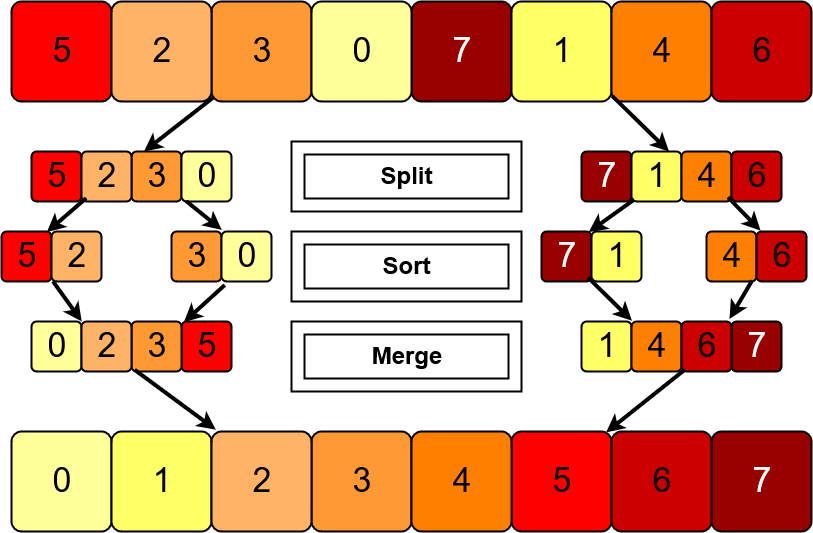
\includegraphics[width=0.45\textwidth]{merge_sort.png}
\caption{Parallel merge-sort algorithm scheme.
Starting from the original array the master thread split the work (sub-arrays) along two slaves threads (\textsf{split} step in the graph).
The split recursion is applied until a required size of sub-arrays is reached.
Each slave-thread applied a sort function (\textsf{sort} step in the graph).
Then the full array is recombined following back the thread recursion applying an \textsf{inplace-merge} function (\textsf{merge} step in the graph).
}
\label{fig:merge_sort}
\end{figure}

As parallelization strategy we can yet invoke the new \emph{keywords} of OpenMP libraries and apply a \emph{divide-and-conquer} architecture using a tree of independent \emph{tasks}\footnote{
  Tasks in OpenMP are code blocks that the compiler wraps up and makes available to be executed in parallel.
}.
Using the maximum power of two of the available threads we split the computation in equal size sub-arrays and perform independent \textsf{argsort}s.
Then, going backwards to the subdivisions at each step we merge the sub-arrays two-by-two until the root.


\end{document}
 % parallel merge-sort
\documentclass{standalone}


\begin{document}

\subsection[Network Signature]{Network signature}\label{implementation:network}

After the rearrangement of feature pairs in ascending order we can start to create the variable network and looking for its connected components as putative signatures.
Each feature will be represent a node in the network and a given pair will be a connection between them.
Since the full storage of the network would require a matrix $(N\times N)$, we have to chose a better strategy for the processing\footnote{
  We are working in the hypothesis of very large $N$.
}.

The ordered set of couples computed in the previous section represents a so-called \emph{COO sparse matrix} (Coordinate Format sparse matrix) and we can reasonable assume that the desired signature will be composed by the top ranking of them.
So, the first step will be to cut a reasonable percentage of the full set of pairs and process only them.

Moreover, we are interested in a small set of variables unknown a prior.
The load of all the node pairs into the same graph can slow down the computation.
An iterative method (with stop criteria) can perform better in the large case of samples and only in worst cases the full set of pair will be loaded.

Since the described algorithm step does not require particular performance efficiency now, the main code used in our simulation was written in pure \textsf{Python}.
A \textsf{C++} implementation of the same algorithm was developed with the help of the Boost Graph Library~\cite{BGL} (BGL), but to not overweight the code installation, it was reserved just for a style exercise.
In this section we discuss about this second version and also about the strategies chosen to implement an efficiency version of it.
This version of the algorithm was also used as stand alone method for other applications that will be presented later.

BGL is a very wide framework for graph analysis based on template structures.
The library efficiency discourage the users to re-implement the same algorithms and, for the current purposes, it was resulted more than sufficient.

Starting from the top scorer feature pairs, we progressively add each couple of nodes to an empty graph.
At each iteration step, the number of connected components is evaluated until a desired number of nodes (greater or equal) is not reached\footnote{
  This procedure is quite similar to put a threshold value on the couple performances or just simpler highlight inside the full network the components linked by weights greater than a given value.
}.
Two degree of freedom are left to the user: in order, \textsf{pruning} and \textsf{merging}.
The first one performs an iteratively remotion of nodes with degree equal (or lower) than 1, i.e pendant nodes, until the graph core is not filtered.
The \textsf{merging} clause choose between the biggest connected component or the the set of all the disjoint connect components as putative signature.
The output of \textsf{merging} step determine the number of nodes in the graph which have been considered for the stop criteria.

A crucial role in the optimization of the algorithm is played by the chosen BGL graph structure.
Since the two degree of freedom imply a continuous rearrangement of the graph nodes, the strategy chosen is to apply a filter mask over the main graph structure that highlights the only part of interest.
This can be done using the \textsf{boost :: filtered\_graph} object of BGL.
In ~\ref{code:featuresel} the \textsf{C++} snippet is shown.

\lstset{style=c++}
\begin{lstlisting}[language=C++, caption=DNetPRO signature extraction, label=code:featuresel]
#include <boost/graph/adjacency_list.hpp>
#include <boost/graph/connected_components.hpp>
#include <boost/graph/filtered_graph.hpp>
#include <boost/function.hpp>
#include <boost/graph/iteration_macros.hpp>

typedef typename boost :: adjacency_list< boost :: vecS, boost :: vecS, boost :: undirectedS, boost :: property< boost :: vertex_color_t, int >, boost :: property < boost :: edge_index_t, int > > Graph;
using V = Graph :: vertex_descriptor;
using Filtered = boost :: filtered_graph < Graph, boost :: keep_all, boost :: function < bool(V) > >;


std :: vector < int > FeatureSelection (int ** couples, const int & min_size, bool pruning=true,  bool merging=true)
{
  Graph G;
  std :: set < V > removed_set;
  Filtered Signature (G, boost :: keep_all {}, [] (V v) {return removed_set.end() == removed_set.find(v);});

  int L = 0, leave, Ncomp, i = 0;

  while ( true ){

    boost :: add_edge (couples[i][0], couples[i][1], G);

    while ( pruning ){

      leave = 0;
      BGL_FORALL_VERTICES (v, Signature, Filtered);
        if ( boost :: in_degree (v, Signature) < 2 ){
          removed_set.insert (v);
          ++ leave;
        }

      if ( leave == 0 )
        break;
    }

    if ( num_vertices (G) - removed_set.size() ){

      components.resize (num_vertices (G));

      Ncomp = boost :: connected_components (Signature, &components[0]);

      if ( merging ){

        BGL_FORALL_VERTICES (v, Signature, Filtered)
          if ( boost :: in_degree(v, Signature) )
            core.push_back ( static_cast < int >(v) );
      }
      else {

        std :: map < int, int > size;
        for ( auto && comp : components ) ++ size[comp];

        auto max_key = std :: max_element (std :: begin(size), std :: end(size),
                                           [] (const decltype(size) :: value_type && p1, const decltype(size) :: value_type && p2)
                                           { return p1.second < p2.second; })->first;

        BGL_FORALL_VERTICES (v, Signature, Filtered)
          if ( components[v] == max_key )
            core.push_back( static_cast < int >(v) );
      }

      components.resize (0);
      L = static_cast < int >(core.size());
    }

    removed_set.clear();

    if ( L >= min_size ) break;

    ++ i;

    core.resize (0);
  }

  return core;
}

\end{lstlisting}

In the above description, it should be clear that, given any set of ordered (in ascending order) couples of variables, this algorithm allows to extract the core network independently by the procedure which generate them.
So it can be used as dimensionality reduction algorithm of general purpose network structures.
An example of this kind of application was reported in Appendix B - Venice Road Network in which we summarized the results of~\cite{Mizzi2018, CurtiSDPS2018}.

\end{document}

 % feat sel algorithm
\documentclass{standalone}


\begin{document}


\subsection[Python wrap]{DNetPRO in Python}\label{implementation:python}

Up to now we are focusing on the algorithm performances leaving out the usability of the DNetPRO algorithm for the (research) community.
Despite the C++ is one of the most efficient and old programming language\footnote{
  Still in common use in scientific research groups.
}, the Python language users are increasing in the last few years.
Python is becoming leader in scientific research publications and the large part of Machine Learning analysis are performed using Python libraries (in particular \emph{scikit-learn} library).
So we have to reach a compromise between the performances and usability of new developed codes and it can be reached using the Cython~\cite{behnel2010cython} framework.

Cython \quotes{language}\footnote{
  It is not a real programming language since it is based on Python.
  However it has its own syntax and keywords which are different either from Python either from C++.
  In the end it needs a compiler to run and it is certainly different from Python.
} allows an easy interface between C++ codes and Python language.
With a relatively simple wrapping of the C++ functions they can be used inside a pure Python code preserving as much as possible the computational performances of the pure C++ version.
In this way we can create a simple Python object which performs the full set of DNetPRO steps and moreover which is compatible with the functions provided by the other machine learning libraries.

With this purposes we chose to operate a double wrap of the C++ functions to separate as much as possible the C++ component from the Python one\footnote{
  Cython wrap are very powerful tools for C++ integration into Python code but, by experience, they are difficult to manage by pure-Python users.
  A simple workaround is to perform a first wrap of the C++ function inside a Cython object and a second wrap of it into a pure-Python one.
  This two-steps wrap certainly gets worse the computational performances but it allows a complete separation between the compiled part of the code (Cython) and the interpreted (Python) one.
  Moreover we can leave back all the checks on input parameters
  in the C++ version since they will be performed at run time in the Python wrap.
}.
The Python object was written considering a full compatibility with the \emph{scikit-learn} library to allow the use of the DNetPRO feature selection as an alternative component of other Machine Learning pipelines.


\end{document}
 % python wrap with sklearn compatibility
\documentclass{standalone}


\begin{document}

\subsection[Pipeline]{DNetPRO in Snakemake}\label{implementation:snakemake}

The starting (silent) hypothesis done until now is that we are running the DNetPRO algorithm on a single dataset (or better on a single Hold-Out subdivision of our data).
On this configuration it is legal to stress as much as possible the available computational resources and parallel processing each step of the algorithm.

If we want to introduce our algorithm inside a larger pipeline, in which we compare the resulting obtained over a Cross-Validation of our datasets we have to re-think about the parallelization done.
In this case, each fold of the cross validation can be interpreted as an independent task and, following the main programming rule \emph{\quotes{parallelize the outer, vectorize the inner}}, we should spawn a thread for each fold and perform the couple evaluation in sequential mode.
Certainly, the optimal solution would be to separate our jobs across a wide range of inter-connected computers and still perform the same computation in parallel but it would required to implement our hybrid (\textsf{C++} and \textsf{Python}) pipeline in a Message Passing Interface (MPI) environment.

An easier solution to overcome all these problems can raise by the use of \textsf{SnakeMake}~\cite{snakemake} rules.
\textsf{SnakeMake} is an intermediate language between \textsf{Python} and \textsf{Make}.
Its syntax is almost like the \textsf{Make} language, but with the help of the easier and powerful \textsf{Python} functions.
It is widely used for bioinformatic pipeline parallelization since it can easily applied over single or multi-cluster environment (master-slave scheme) with a simple change of command line.

\begin{center}
\begin{figure}[htbp]
\hspace{-2cm}
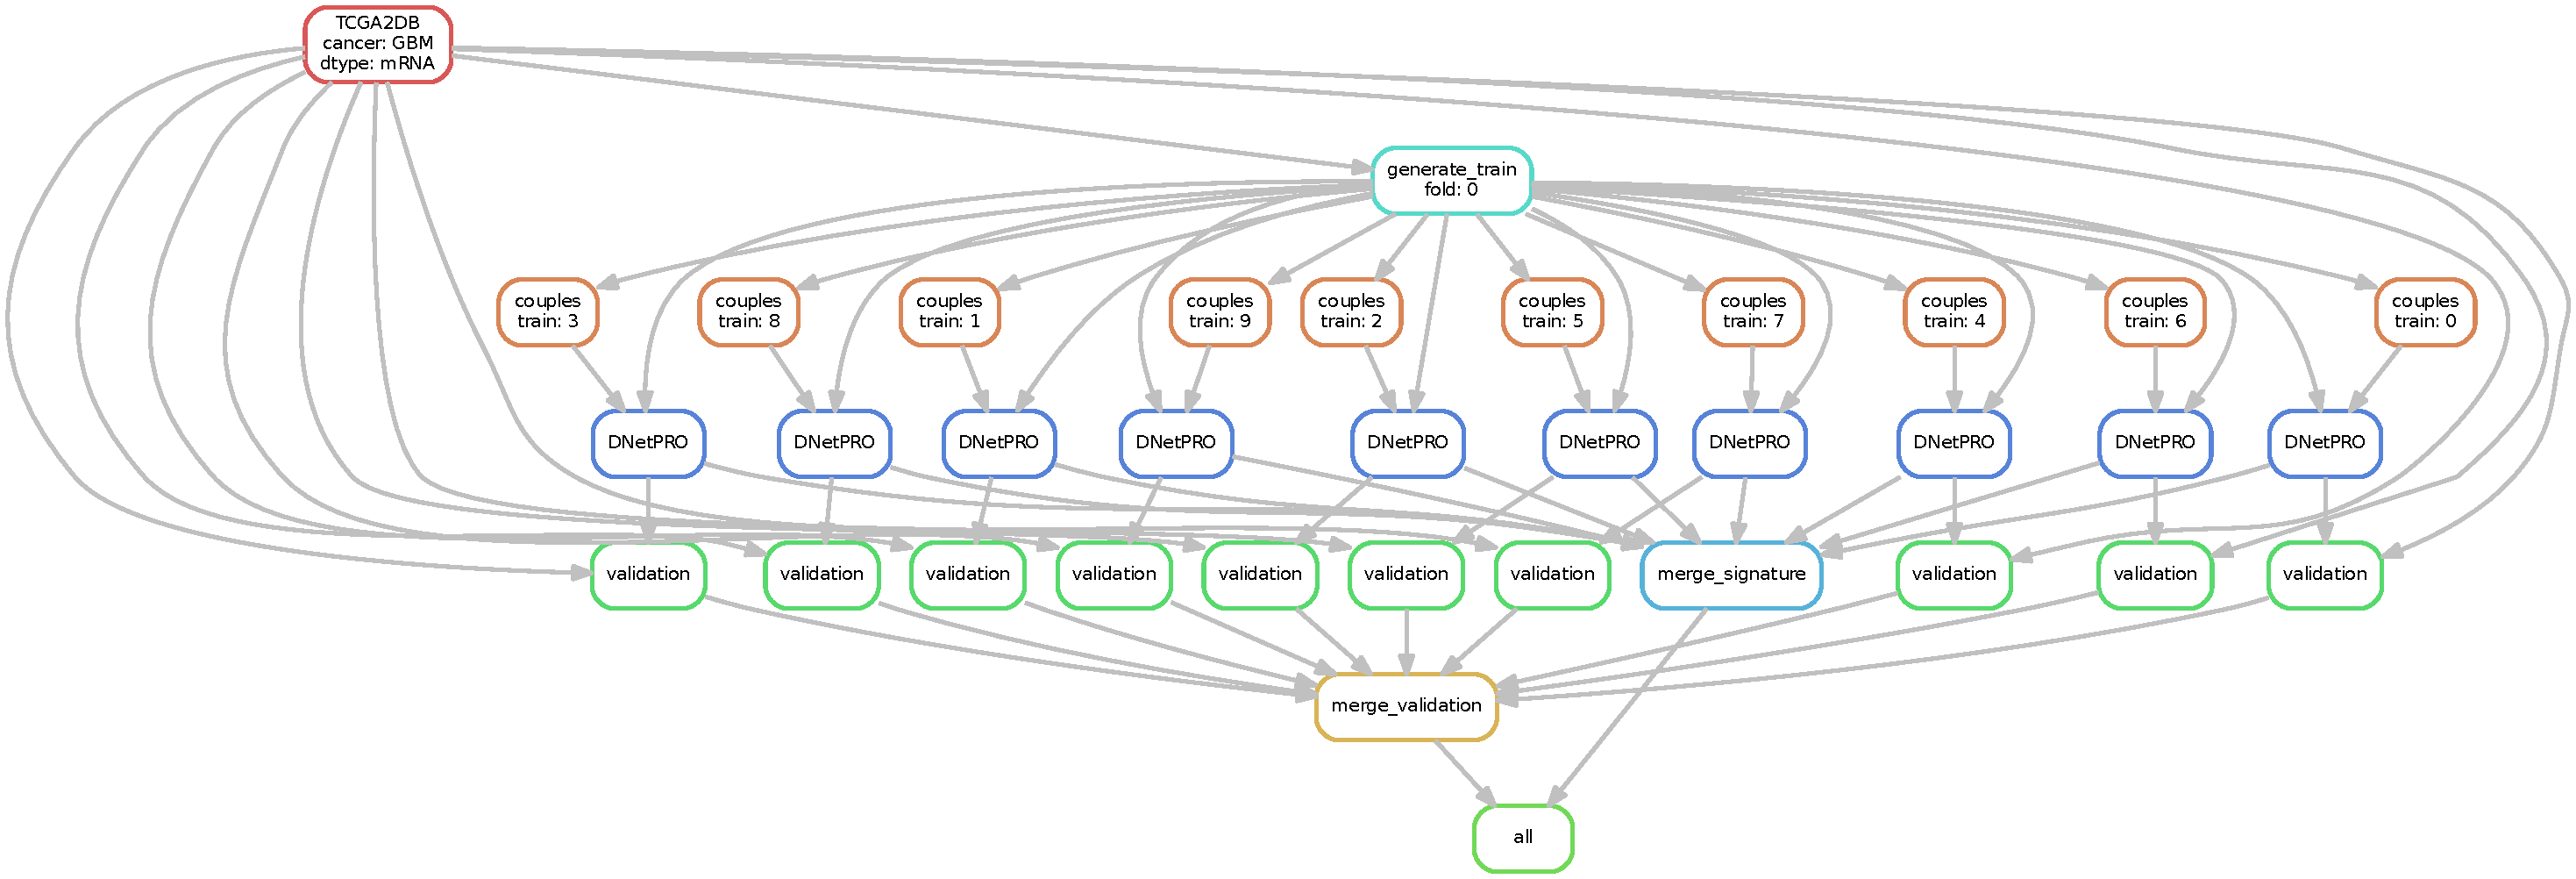
\includegraphics[width=1.3\textwidth]{qdanet_pipe_single.pdf}
\caption{Example of DNetPRO pipeline on a single cross validation.
It is highlighted the independence of each fold from each other.
This scheme shows a possible distribution of the jobs on a multi-threading architecture or for a distributed computing architecture.
The second case allows further parallelization scheme (hidden in the graph) for each internal step (e.g. the evaluation of each pair of genes).
}
\label{fig:dnet_workflow}
\end{figure}
\end{center}

So to improve the scalability of our algorithm we implement the benchmark pipeline scheme using Snakemake rules and a work-flow example for a single cross-validation is shown in Fig.~\ref{fig:dnet_workflow}.
In this case each step of Fig.~\ref{fig:dnet_workflow} can be performed by a different computer unit preserving the multi-threading steps, with a maximum scalability and the possibility to enlarge the problem size and the number of variables.


\end{document}
 % pipeline description with snakemake
\documentclass{standalone}


\begin{document}

\subsection[Time performances]{Time performances}\label{implementation:timing}

As described in the above sections the DNetPRO is a combinatorial algorithm and thus it requires a particular accuracy in the code implementation to optimize as much as possible the computational performances.
The theoretical optimization strategies described until now have to be proofed by quantitative measures.

We tested the computational performances of our Cython (C++ wrap) implementation against the pure Python (naive) implementation shown in \ref{code:py_couples}.
The time evaluation was performed using the \textsf{timing} Python package in which we can easily simulate multiple run of a given algorithm\footnote{
  We would stress that we can use the \textsf{timing} Python package only because we provided a Cython wrap of our DNetPRO algorithm implementation.
  We would also highlight that, albeit minimal, the Python superstructure penalizes the computational performances and the best results can be obtained using the pure C++ version of the code.
}.
In our simulations we monitored the three main parameters related to the algorithm efficiency: the number of samples, the number of variables and (as we provided a parallel multi threading implementation) the number of threads used.
For each combination of parameters we performed 30 runs of both algorithms and we extracted the minimum execution time.
The tests were performed on a classical bioinformatics server (128~GB RAM memory and 2 CPU E5-2620, with 8 cores each)
The obtained results are shown in Fig.~\ref{fig:dnetpro_timing}.
In each plot we fixed two variables and we evaluated the remaining one.

\begin{figure}[htbp]
\def\svgwidth{0.4\textwidth}
\input{./img/features_timing.pdf_tex}
\qquad\qquad
\centering
\def\svgwidth{0.4\textwidth}
\input{./img/samples_timing.pdf_tex}
\qquad\qquad
\centering
\def\svgwidth{0.5\textwidth}
\input{./img/nth_timing.pdf_tex}
\caption{Execution time of DNetPRO algorithm.
We compare the execution time between pure-Python and Cython (C++ wrap) implementation.
\textbf{(a - left)} Execution time in function of the number of variables (the number of samples and the number of threads are kept fixed).
\textbf{(b - right)} Execution time in function of the number of samples (the number of variables and the number of threads are kept fixed).
\textbf{(c - bottom)} Execution time in function of the number of threads (the number of variables and the number of samples are kept fixed).
}
\label{fig:dnetpro_timing}
\end{figure}

In all our simulations the efficiency of the (optimized) Cython version is easily visible and the gap between the two implementations reached more than $10^4$ seconds.
On the other hand is important to highlight the scalability of the codes against the various parameters.
While the code performances scales quite well with the number of features (Fig.~\ref{fig:dnetpro_timing}(a)) in both the implementations, we have a different trend varying the number of samples (Fig.~\ref{fig:dnetpro_timing}(b)): the Cython trend starts to saturate almost immediately while the computational time of the Python implementation continues to grow.
This behavior highlights the results of the optimizations performed on the Cython implementation which allows the application of the DNetPRO algorithm also to larger datasets without loosing performances.
An opposite behavior is found monitoring the number of threads (ref Fig.~\ref{fig:dnetpro_timing}(c)): the Python version scales quite well with the number of threads\footnote{
  The optimal result should be a linear scalability with the number of threads but it is always difficult to reach this efficiency.
  Thus, a reasonable good result is given by a progressive decrease with increasing the number of threads.
}, while Cython trend is more unstable.
This behavior is probably due to a not optimized schedule in the parallel section: the work is not equally distributed along the available threads and it penalizes the code efficiency creating a bottleneck related to the slowest thread.
The above results are computed considering a number of features equal to 90 and thus the parallel section distributes the 180 ($N\times N$) iterations along the available threads: when the number of iterations is proportional to the number of threads used (12, 20 and 30 in our case) we have a maximization of the time performances.
Despite this, the computational efficiency of the Cython implementation is so better than the Python one that its usage is indisputable.

\end{document}
 % timing performances

\documentclass{standalone}

\begin{document}

\section[Benchmark]{Benchmark of DNetPRO algorithm}\label{synapse:benchmark}

Up to now we have been talked about the DNetPRO algorithm from a theoretical point-of-view.
Starting from this section we discuss about the application of the algorithm on real biological datasets (see Appendix B - Venice Road Network for results obtained on a different kind of data).

Despite previous version of the DNetPRO method were already applied on biological data~\cite{PMrna, Scotlandi2009, PMgene, Terragna} a wide range benchmark of it was still missing.
In the following sections we describe the results obtained on the Synapse dataset and published in~\cite{Curti2019}.

\end{document}
 % Introduction ot TCGA dataset
\documentclass{standalone}

\begin{document}

\subsection[Synapse]{Synapse dataset}\label{synapse:synapse}

As benchmark dataset was chosen the core sets extracted from the The Cancer Genome Atlas (accession number \href{https://www.synapse.org/#!Synapse:syn300013/wiki/27406}{syn300013, doi:10.7303/syn300013}) (\emph{Synapse dataset} in the following), used in a previous study~\cite{Yuan2014} which aimed at quantifying the role of different omics data types (e.g. mRNA and miRNA microarray data,  protein levels measured with Reverse Phase Protein Array - RPPA) via different state-of-the-art classification methods.
This allowed us to compare our results to a large set of commonly used classification methods, by using their performance validation pipeline (accession number \href{https://www.synapse.org/#!Synapse:syn1710282/wiki/27303}{syn1710282, doi:10.7303/syn1710282}).

The Synapse dataset is composed by four tumors datasets: kidney renal clear cell carcinoma (KIRC), glioblastoma multiforme (GBM), ovarian serous cystadenocarcinoma (OV) and lung squamous cell carcinoma (LUSC).
For each cancer type we applied the \textsf{DNetPRO} algorithm on mRNA, miRNA and RPPA data and we compare the performances results with the Yuan et al. ones.

The summary description of the datasets used is reported in the Tab.~\ref{tab:synapse}.

\begin{table}[htbp]
\centering
\begin{tabular}{lccccccc}
\hline \rowcolor{darkgrayrow}
         &               &                &          & Number       \\
\rowcolor{darkgrayrow}
Cancer   & mRNA          & miRNA          & Protein  & of samples   \\
\hline
GBM      & AgilentG4502A & H-miRNA\_8x15k & RPPA     &              \\
         & 17814         & 533            & $^a$     & 210          \\
KIRC     & HiseV2        & GA+Hiseq       & RPPA                    \\
         & 20530         & 1045           & 166      & 243          \\
OV       & AgilentG4502A & H-miRNA\_8x15k & RPPA     &              \\
         & 17814         & 798            & 165      & 379          \\
LUSC     & HiseqV2       & GA+Hiseq       & RPPA     &              \\
         & 20530         & 1045           & 174      & 121          \\
\hline
\end{tabular}
\caption{In the first row platforms are reported and the second shows the dimension of dataset as number of probes.
AgilentG4502A: Agilent 244K Custom Gene Expression G4502A;
HiseqV2: Illumina HiSeq 2000 RNA Sequencing V2;
H-miRNA\_8x15K: Agilent 8~×~15K Human miRNA-specific microarray platform;
GA+Hiseq: Illumina Genome Analyzer/HiSeq 2000 miRNA sequencing platform;
RPPA: MD Anderson reverse phase protein array.
The last column shows the number of sample.
\newline $^a$ Missing data-type for that cancer type.
}
\label{tab:synapse}
\end{table}

Each tumor dataset was pre-processed by adding a zero-mean Gaussian random noise ($\sigma = 10^{-4}$)) to remove the possible null values in the database, which could produce numerical errors in the distances evaluation between genes.
Then, we randomly split each dataset in training and test sets with a stratified (i.e. balanced for class sample ratio) 10-fold procedure: with the stratification we are reasonably sure that each training-set is a good representative of the whole sample set.
The choice of a 10-fold splitting is aimed to reproduce the analysis pipeline presented by Yuan et al. with an analogous cross-validation procedure.
Since we don't have exact details of their data splitting, the cross validation was repeated 100 times, for a total of 1000 training procedures for each tumor (OV, LUSC, KIRC, GB) and data type (mRNA, miRNA, RPPA).
Each training procedure led to the extraction of multiple signatures.

We chose threshold values in order to obtain a resulting number of variables (network nodes) in the order of $10^2-10^3$, and identified all connected components of the network as signatures.
If more than one component existed, each one was considered as a different signature.

The final multidimensional signatures were tested by a Discriminant Analysis with a diag-quadratic distance, to avoid possible problems about covariance matrix inversion (as for the Mahalanobis distance).

\begin{center}
\begin{figure}[htbp]
\centering
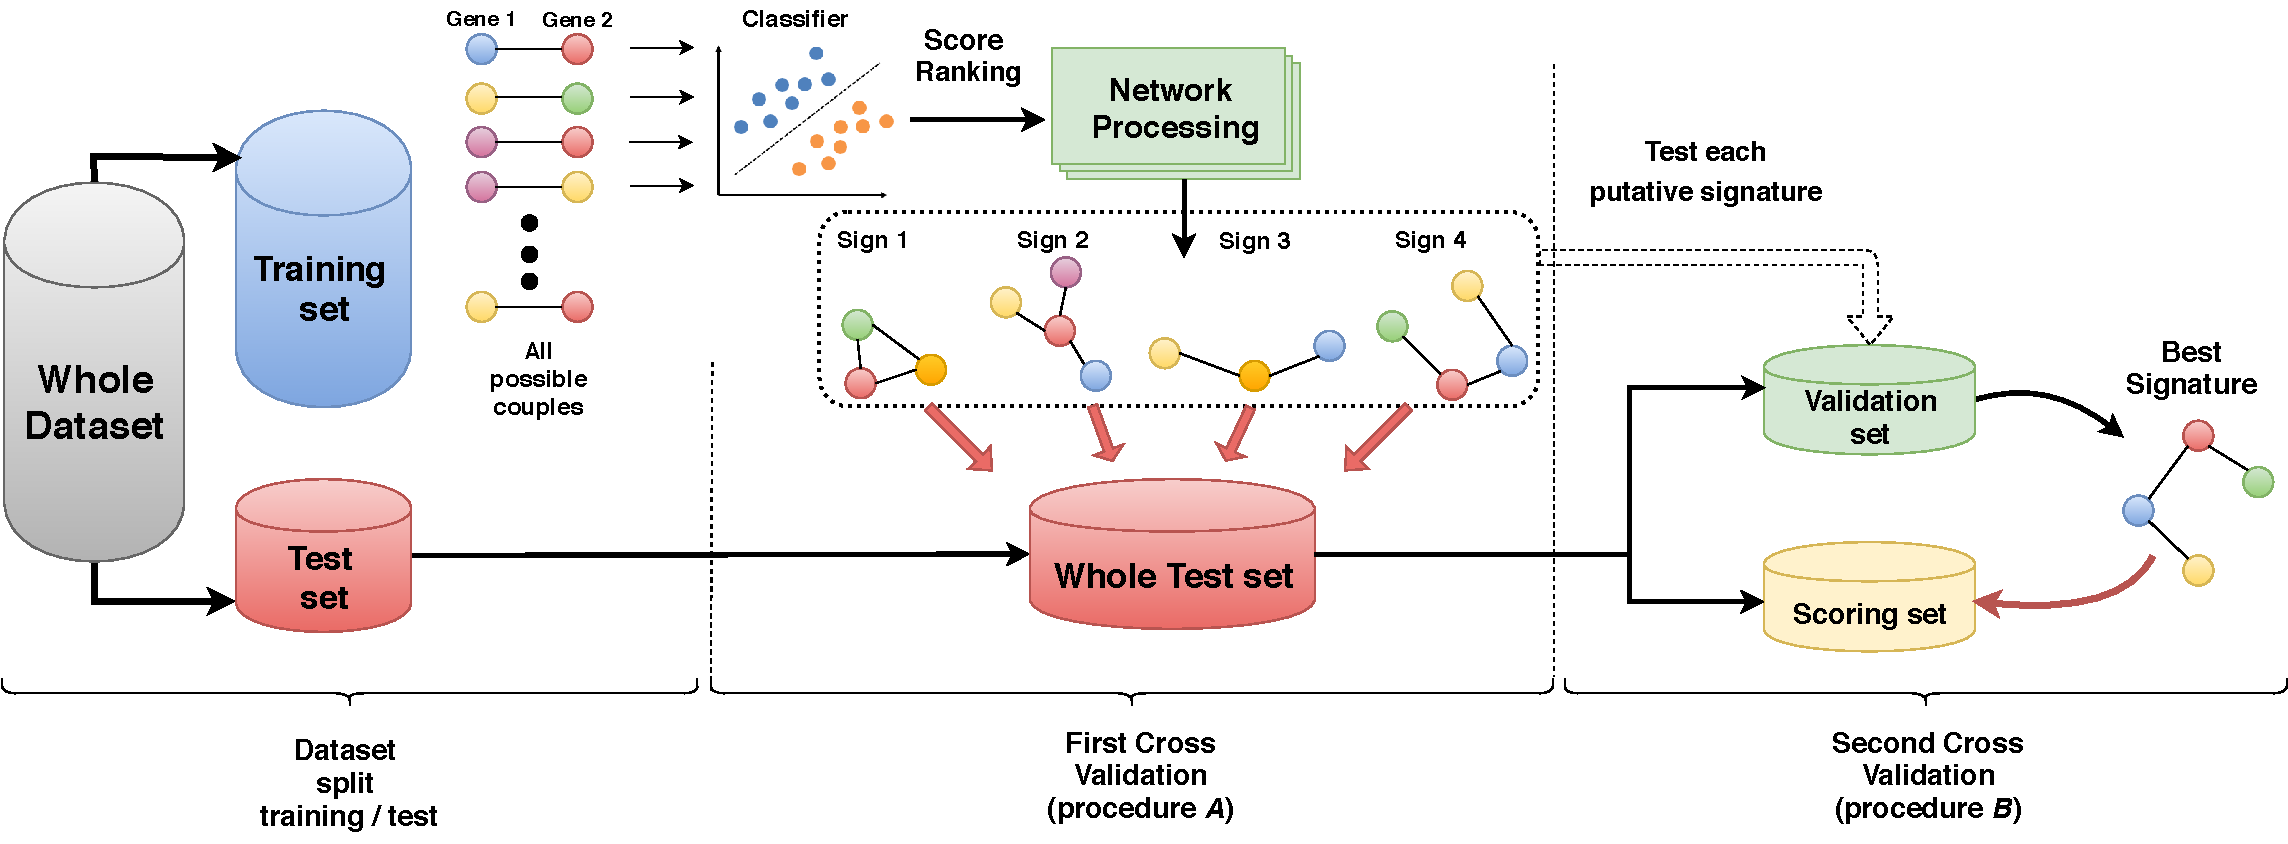
\includegraphics[width=1.0\textwidth]{dnet_pipe.pdf}
\caption{Scheme of \textsf{DNetPRO} algorithm.
On the \quotes{training set}, all possible couples of variables are used for Discriminant Analysis, generating the fully connected network weighted by classification performance.
Thresholding ranked couples, several signatures can result (as connected components) and their performance is evaluated on the \quotes{whole test set} (procedure $A$).
% Signatures are given by the connected components created by all couples with scorer greater than a chosen threshold.
A unique best signature can be identified on a \quotes{validation set} and tested in a \quotes{scoring set}, obtained by further splitting the \quotes{whole test set} (procedure $B$).
% The pipeline parameters was adapted to faithfully mimic the reference work-flow to allow a comparison of the final results except for the second cross validation step.
}
\label{fig:dnet_pipe}
\end{figure}
\end{center}

We remark that \textsf{DNetPRO} can provide more than one signature as a final outcome, given by all the connected components found in the variable network, or a unique top-performing signature can be obtained by a further cross-validation step (procedure $A$ and procedure $B$ in Fig.~\ref{fig:dnet_pipe}, respectively).

In the single cross validation configuration (procedure $A$ in Fig.~\ref{fig:dnet_pipe}), the best signature was extracted as the one reaching the highest accuracy score during the training step.
This best signature was then tested over the available test set.

When also the second cross validation was used (procedure $B$ in Fig.~\ref{fig:dnet_pipe}) the best signature wasted as the most performing over a subset of the whole test set (\emph{validation set}), and the final performance was evaluated on the remaining \emph{scoring set}.

To compare our results with the work of Yuan et al., we used the AUC (\emph{Area Under the Curve}) score, that they provided in the paper as the result of their analyses.
The distribution of our results could be compared to the single score value given in the other work.

\end{document}
 % dataset description
\documentclass{standalone}

\begin{document}

\subsection[mRNA data]{mRNA dataset}\label{synapse:mRNA}

We applied both training procedure (ref.~\ref{fig:dnet_pipe}) on the mRNA dataset.
The results are shown, as distribution of AUC (Area under the curve) score, in Fig.~\ref{fig:dnet_results}~(a) for the best signatures obtained with procedure $A$ (corresponding to the validation approach used in~\cite{Yuan2014}), while results with the full cross-validation procedure $B$ are shown in Fig.~\ref{fig:dnet_results}~(b).

As expected, performances decrease with the introduction of the second cross validation step, but the values remain quite stable showing the robustness of the extracted signatures, and we remark that the validation procedure used in the reference paper by Yuan et al. resembles our approach without the second validation step.

\begin{figure}[htbp]
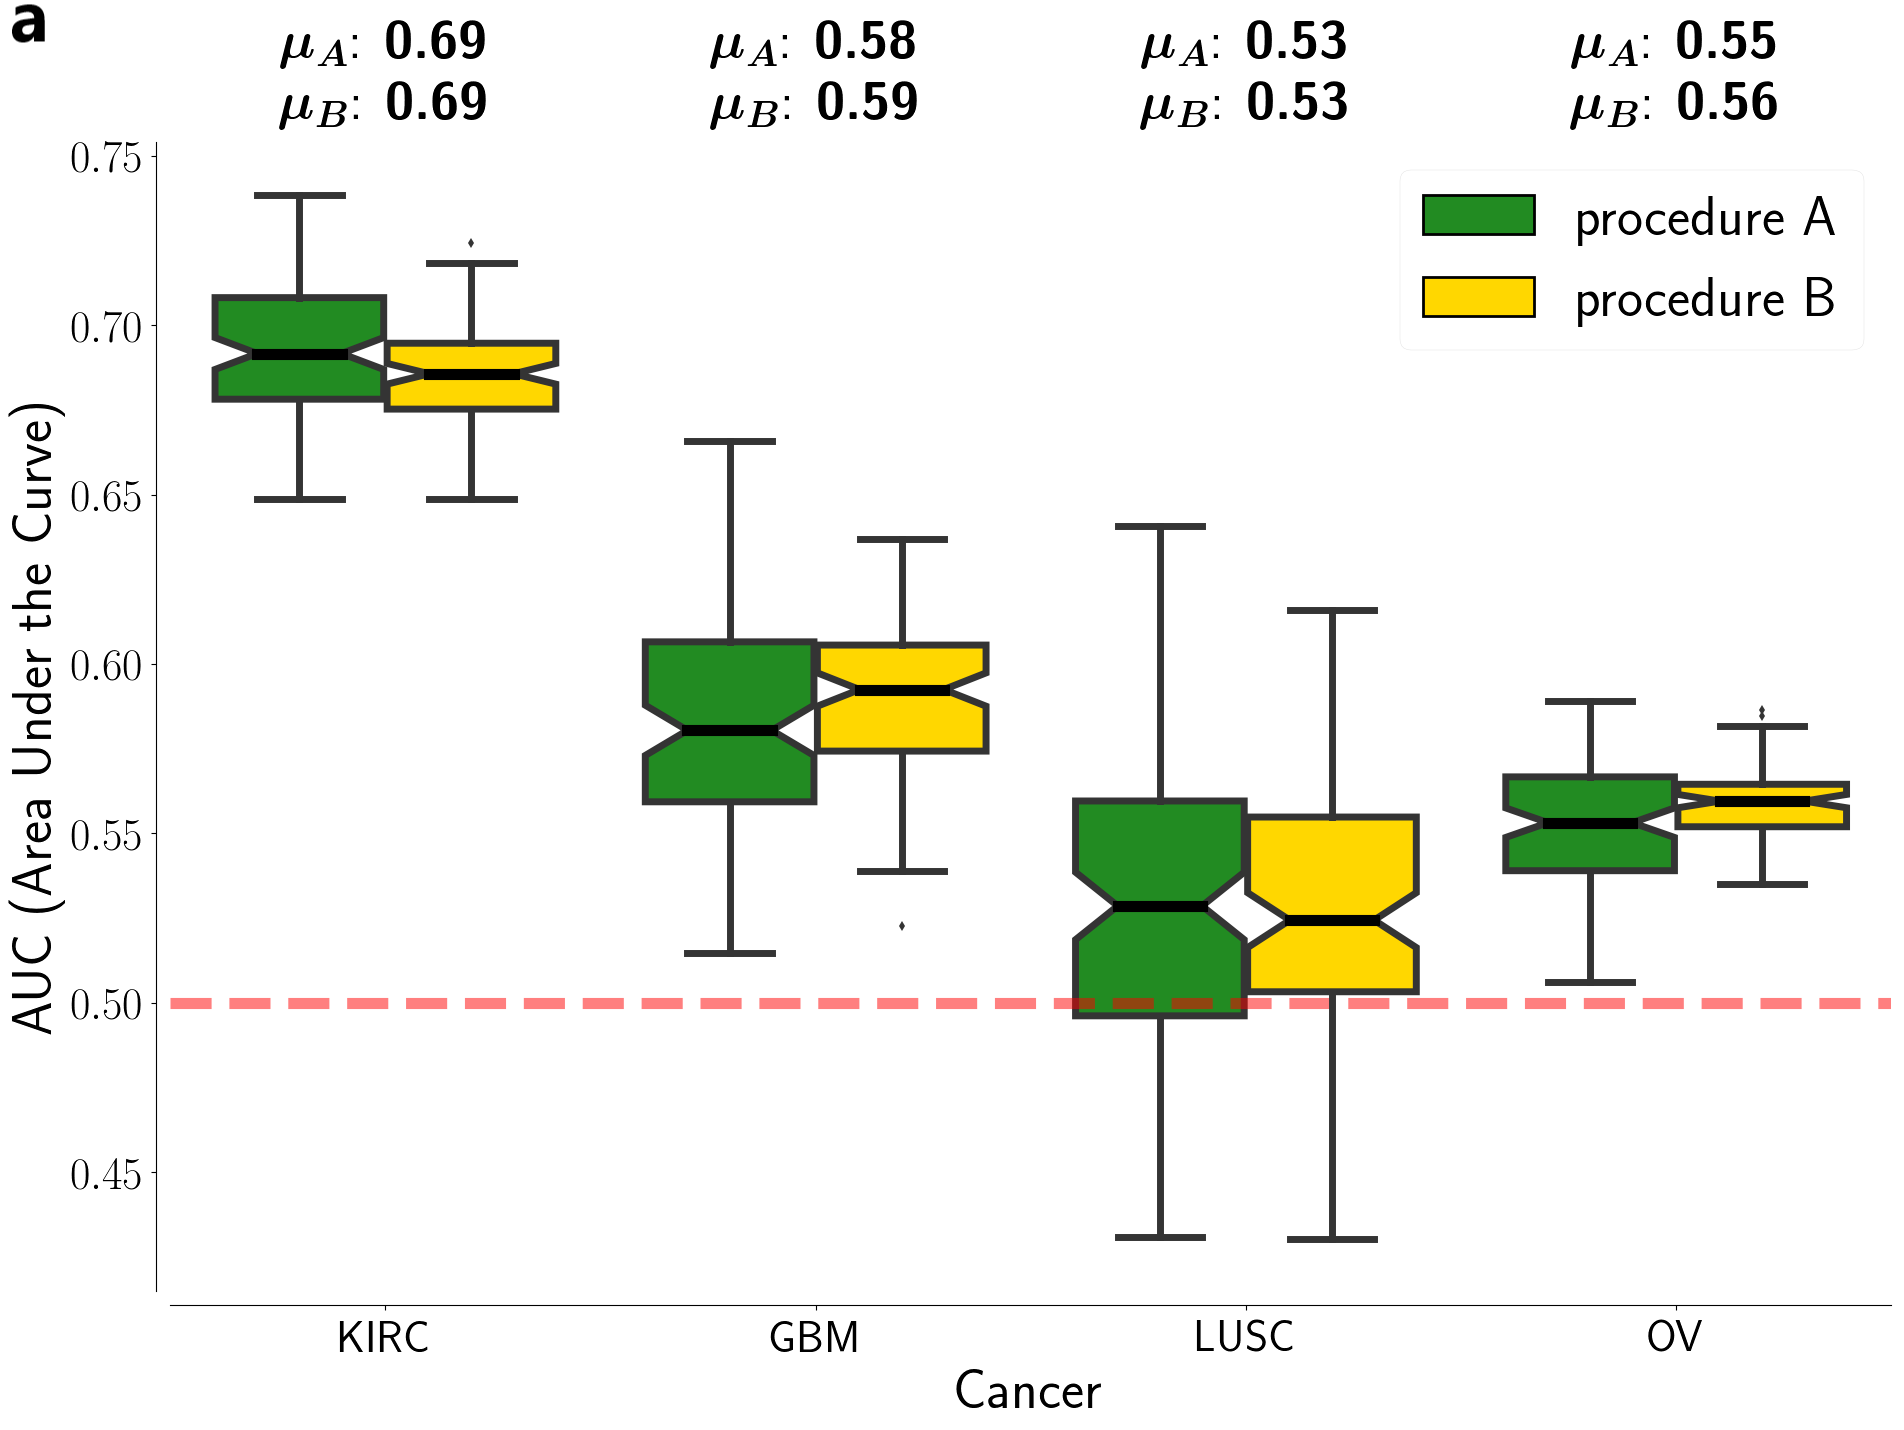
\includegraphics[width=0.4\textwidth]{mRNA_boxplot.png}
\qquad\qquad
\centering
\def\svgwidth{0.45\textwidth}
\input{./img/mRNA_tables.pdf_tex}
\caption{Results obtained by the DNetPRO algorithm pipeline on four mRNA tumor datasets, as from the Synapse database~\cite{Yuan2014}.
\textbf{(a)} Distributions of AUC values for the tumor datasets. Green boxplots: results using procedure $A$ as described in Fig.~\ref{fig:dnet_pipe}; yellow boxplots: results obtained using procedure $B$.
\textbf{(b)} Comparison of DNetPRO results with the methods used in the paper of Yuan et al.: max AUC values obtained over the 10-Fold cross-validation procedure.
}
\label{fig:dnet_results}
\end{figure}

All results are comparable (LUSC) or better (KIRC, GBM) than the results reported in~\cite{Yuan2014}, except for the OV dataset, also with the more conservative approach involving a further cross-validation step.
The size of the extracted signatures is quite constant, and smaller than 500 genes in each pipeline execution.
Analogous results are obtained also for the miRNA dataset, in which our method outperforms in three over four cases, while the RPPA dataset shows less significant results (Supplementary material).

To test the robustness of our method, since each cross-validation procedure may generate different signatures, we measured the overlap of the genes belonging to each mRNA signature over 100 simulations with different training-test data splitting.
We observed an average overlap ranging from 40\% to 60\%, with a smaller group of genes found across all the 100 cross-validation iterations.

In this application the DNetPRO algorithm has several advantages: easy scalability on parallel architectures, simple signature interpretation allowing a valuable application in a biomedical context and a significant robustness in a highly noisy environment such as genomics measurements.

\end{document}
 % mRNA results
\documentclass{standalone}

\begin{document}

\subsection[miRNA and RPPA data]{miRNA and RPPA dataset}\label{miRNA}

\end{document}
 % miRNA and RPPA results
\documentclass{standalone}

\begin{document}

\subsection[Ranking]{Couple ranking}\label{synapse:ranking}

Since the number of variable pairs is typically very large (e.g. $10^8$ pairs with gene expression microarrays containing about $10^4$ probes) many of them may achieve the same performance, since the possible performance values are integer number typically in a limited range (corresponding to the number of available samples, $10^2-10^3$ in many cases).
Therefore, the ranking of pairs by their performance is characterized by multiple \quotes{plateaus}(Fig.~\ref{fig:plateaus}(a)), and the selection of probe pairs based on a hard thresholding procedure is highly influenced by this feature.
Monitoring this trend behavior can be noticed that only a few number of pairs belongs to the first performances chunks and while the performances decrease multiple pairs and features appear, as it can be seen in Fig.~\ref{fig:plateaus}(a).

This kind of trend highlight the difficulty on finding informative features inside the huge noise of other variables and it gives us a constrain in the developing of a realistic biological toy model.
Moreover it confirms us that a putative signature could be made by only a few amount of central genes at least weakly connected with other noise nodes.

\begin{figure}[htbp]
\centering
\def\svgwidth{0.4\textwidth}
\input{./img/lengths.pdf_tex}
\qquad\qquad
\def\svgwidth{0.4\textwidth}
\input{./img/plateaus.pdf_tex}
\caption{Analysis of ranked pairs distributions according to the performance score obtained in the training step.
(\textbf{a}) The distribution of plateau lengths is approximately exponential.
(\textbf{b}) Average number of pairs with the same score value: this behavior is typical in ranking order distribution and it can be fitted by the relation $f(x) = A(M + 1 - r)^b / r^a$ as shown in~\cite{rankfit}, where $r$ is the rank value, $M$ its maximum value, $A$ a normalization constant and ($a$, $b$) two fitting exponents.}
\label{fig:plateaus}
\end{figure}

As in other cases of ranked values~\cite{rankfit}, we can fit these ranking distributions with a combination of power-law functions obtaining a good agreement with experimental points (Fig.~\ref{fig:plateaus}(b)).

We also observed that \emph{star}-networks frequently appear, with one variable highly connected to many others which are only connected with it.
This happens when a variable has a strong discriminating power, to which other possibly less relevant variables get linked for noisy fluctuations.

As stated before, we suggest that these variables (pendant nodes in the star network) can be removed from the signature without significantly affecting its performance.
The procedure can be applied for one single step (in order to remove nodes pending from a star configuration) or it can be applied recursively, until the signature becomes constituted only by the 2-core network (i.e. with all nodes having degree $\geq2$).
Empirical analysis performed on real data has shown that the removal of these variables does not affect significantly the signature performance, and in the meanwhile it allows a significant reduction of its dimensionality.
Since there is no clear theoretical explanation of this behavior, we suggest to introduce this step only optionally, since it is not easy to quantify the risk of loosing relevant information from the removed variables.

The underlying idea is that the more connected are the nodes, the more the variables in the signature \quotes{work well} together, a plausible hypothesis given the linear sample separation surface provided by the Discriminant classifier.
Moreover, the network structure of the signature suggests further considerations about the relevance of a variable as a function of its role in the network (e.g. node centrality such as degree or betweenness centrality).

\end{document}
 % ranking couples conclusions
\documentclass{standalone}

\begin{document}

\subsection[Signature Overlap]{Characterization of signature overlap}\label{synapse:overlap}

In the analysis of the Synapse dataset we used a complex pipeline of cross-validation (ref Fig.~\ref{fig:dnet_pipe}) to obtain a sufficient statistics.
The DNetPRO algorithm was designed to work on a single dataset since the signature extraction can involve different variables for different data subdivisions.
In our application we divide the dataset into a training-test subdivision and the signature were extracted along a 10-fold cross-validation over the training set.
This kind of setup could produce 10 totally different signatures, in the worst case.
Moreover we replicated our simulation for 100 repetitions and thus a set of 1000 totally independent signatures were extracted.

Starting from this large subset of variables we can evaluate the robustness of the DNetPRO algorithm in the variable identifications studying the overlap between these signatures.
From a statistical point-of-view is quite unlikely that the same set of variables were included into all the extracted signatures, especially on this application, in which the variable roles are assumed by genes.
On the other hand the overlap of these signatures could highlight a statistical significance of some variables and thus genes related to the understudied tumors.

As case study we analyzed only the KIRC mRNA dataset in which the extracted signatures ranged from 4 to 650 genes ($\mu=382$ genes).
For each gene we counted its occurrences along the 1000 signatures.
The same analysis was performed taking into account the signatures generated using the $K$-best score variables (ref.~\ref{dnetpro:toy} for further informations) and a random features extraction.
In Fig.~\ref{fig:overlap} the genes distribution obtained by the three methods are shown.

\begin{figure}[htbp]
\centering
\def\svgwidth{0.6\textwidth}
\input{./img/DNetPRO_overlap.pdf_tex}
\caption{Signatures overlap obtained in the KIRC mRNA datasets.
Genes occurrences of the 1000 DNetPRO signatures extracted from the Synapse pipeline (blue).
Genes occurrences of the 1000 $K$-best variables extracted from the Synapse pipeline (red): the number of genes ($K$) is the same of the corresponding DNetPRO signature.
Genes occurrences of 1000 random signatures (yellow).
}
\label{fig:overlap}
\end{figure}

Both DNetPRO and $K$-best feature extraction algorithms identified a core set of genes common to the full set of signatures.
The $K$-best algorithm appears more stable than the DNetPRO algorithm and it is easier to find the same genes along the extracted signatures.
This behavior could be associated to the problems highlight also in the toy model simulations (ref. \ref{dnetpro:toy}): the DNetPRO algorithm is able to identify only one signature but the informative features (genes) could not co-operate in the same network-signature and thus they could be discarded.
The DNetPRO signatures are, in fact, very small compared to the number of variables and thus only small network components were extracted which are very closed to star-networks.
Despite the discrepancy between the signatures we have a core of 18 genes which occurs in at least the 95\% of both signatures and 8 of them are in the 99\% of both signatures.

The common genes were also mapped on public databases (TISIDB~\cite{10.1093/bioinformatics/btz210} and Oncotarget~\cite{
%TODO:MISS REF (search KIRC LTB4R on google)
}, which link tumors to related genes.
We found 14/18 genes as informative probes for the KIRC tumor in the TISIDB and 7 of them were also found in the Oncotarget database\footnote{
  The list of genes in the TISIDB cover \quotes{only} 988 genes.
  From our list we have only one gene which was found in the Oncotarget database and not in the TISIDB.
  This gene misses in the TISIDB so we can not evaluate its importance.
}.
Taking into account the core set of 8 genes we found 3 of them on Oncotarget database and 7 of them on the TISIDB.
The only exception was given by the LOC388796 gene which was not found in any database.

The random feature extraction method is not even comparable with the others and it simply represents a null model.

\end{document}
 % overlap of signatures

\documentclass{standalone}

\begin{document}

\section[Cytokinoma Dataset]{Cytokinoma dataset}\label{cytokine}

Increasing evidence suggests that inflammation is involved in Alzheimer's disease (AD) pathogenesis.
Elevated peripheral levels of different cytokines and chemokines in subjects affected by AD compared with healthy control (CTL) have emphasized the role of peripheral inflammation in the disease.
Thus, these proteins can represent specific factors of disease development and progression.
Considering the cross-talking between the central nervous system and the periphery, the inflammatory analytes may provide utility as biomarkers to identify AD at earlier stages, in particular for the diagnosis of Mild Cognitive Impairment (MCI), a condition at risk of development of dementia.
AD is a major neurocognitive disorder and the most common cause of dementia in the old age, accounting for 60\% to 80\% of all causes.
During the past decade, a conceptual shift occurred in the field of AD considering the disease as a continuum.
In this context, there is an urgent need for biomarkers identification able to accurately detect AD in an early stage, before the appearance of neurologic signs.
An early diagnosis can hopefully lead to a better and more effective treatment, which could potentially limit neuronal damage and prevent the development of overt AD.
An emerging field in the study of neuroinflammation is the sex-related differences: in the last years, gender studies have been increasingly developed with the aim to adopt gender differences as a key to interpretation many diseases, including neurodegenerative diseases.

Experimental data showed that many mechanisms are involved in AD pathogenesis including neuroinflammation.
The dysregulation of cytokines and chemokines is a central feature in the development of neuroinflammation, neurodegeneration, and demyelination both in the central and peripheral nervous systems.
Among many chemokines and cytokines, pro-inflammatory IFN$\alpha$2, TNF$\alpha$, and IL-1$\alpha$ are described as heterogeneously implicated in AD pathogenesis.

The interactive network of cytokines/chemokines, defined as \quotes{cytokinome}, is extremely complex.
Using the DNetPRO algorithm as statistical feature selection method, we might discriminate the groups and propose a useful tool to follow the progression and evolution of AD from its early stages, also in light of gender differences.
With this study, we aimed first at the identification of a potential proteins profile able to discriminate AD, MCI and CTL and, therefore identify a potential early and easy to get a diagnostic marker of subjects at risk.

\end{document}
 % Introduction to Cytokine
\documentclass{standalone}

\begin{document}

\subsection[Dataset]{Dataset}\label{cytokine:cytokine_data}

In this case-control observational study, we evaluated $289$ old-age subjects referred to our Geriatric Memory Clinic.
The dataset comprises $189$ female and $100$ male individuals with a mean age of $78.6$ ($\pm7.5$) years.
The date were provided by the co-authors of this project at the Institute of Gerontology and Geriatrics at the University of Perugia (Department of Medicine).
For each patient a set of 26 cytokine expression level were computed with the additional information about subject sex, age and diagnosis label (AD, MCI or CTL).
Of the 289 enrolled subjects, the whole set of cytokines was available for 284 subjects (98\%), specifically 87/88 CTL (99\%), 70/73 MCI (96\%), 127/129 AD (98\%).

To approximate normal distribution, plasma cytokines and chemokines were log-transformed for data analyses.
For the analysis of single cytokines with respect to the CTL, MCI and AD group, we designed a linear model analysis, with the value of each cytokine as a linear combination of the subject group (with CTL samples as the baseline, and MCI, AD as conditions), age and sex, as factors (the formula representation would be \quotes{cytokine $\sim$ group + sex + age}).
The last two were included as possible confounding factors, even if the analyses revealed that their role for each cytokine is marginal.
Only IFN$\alpha$2, IL-1$\alpha$, and MCP-1 differed among groups after correction for age and sex.
A threshold $p<0.05$ was considered for significance at all levels (group, sex or age).

Then we applied the \textsf{DNetPRO} algorithm looking for a signature capable of discriminating between CTL and AD: to this purpose, we performed a Hold-Out cross-validation procedure to identify the cytokine signature, considering 2/3 of samples to train the model and then we tested the signature performance on the remaining 1/3 of the total samples.
In this analysis we did not separate male from female samples, to avoid the bias given by the uneven number of samples in these two groups, and since previous analysis at a single-cytokine level did not find significant differences due to sex.
Then, we classified MCI samples with the CTL-AD signature obtained in the previous step, that allowed labeling MCI samples as CTL or non-CTL.

%Description of the cytokinoma dataset with statistics.
%Application of the \textsf{DNetPRO} on the Cytokine dataset.
%Discussion on the obtained signature and biological %interpretation of the Alzheimer disease.


\end{document} % Dataset description
\documentclass{standalone}

\begin{document}

\subsection[Results]{Resuls}\label{cytokine:cytokine_result}

The best signature identified to discriminate between CTL and AD subjects is composed of three cytokines, IFN$\alpha$2, TNF$\alpha$, and IL-1$\alpha$.
Its total accuracy on the CTL-AD test set is 65.27\% (with 61\% CTL and 66\% AD correctly classified).
The sensitivity/specificity values for classification is reported in Tab.~\ref{tab:cytokine}.

\begin{table}[!htb]
  \begin{minipage}{.5\linewidth}
    \hspace{-1.5cm}
      \begin{tabular}{cccc}
          \hline \rowcolor{darkgrayrow}
                      &  \textbf{Accuracy}  &  \textbf{Sensitivity}  &  \textbf{Specificity} \\
                      &  AD vs. CTL         &  AD                    &    CTL                \\
          \hline
              Men     &    16/25            &    8/12                &    8/13               \\
                      &          (64.00\%)  &         (66.67\%)      &         (61.54\%)     \\
              Women   &    33/48            &   27/38                &    6/10               \\
                      &          (68.75\%)  &         (71.05\%)      &         (60.00\%)     \\
              Total   &    47/72            &   36/54                &   11/18               \\
                      &          (65.24\%)  &         (66.66\%)      &         (61.11\%)     \\
          \hline
      \end{tabular}
  \end{minipage}%
  \begin{minipage}{.5\linewidth}
    \hspace{.5cm}
      \begin{tabular}{ccc}
          \hline \rowcolor{darkgrayrow}
                        \textbf{Prediction} &  \textbf{Sensitivity}  &  \textbf{Specificity} \\
                         MCI as non-CTL     &  MCI                   &    CTL                \\
          \hline
                           15/26            &   15/26                &   24/36               \\
                                 (57.69\%)  &         (57.69\%)      &         (66.67\%)     \\
                           41/47            &   41/47                &   23/51               \\
                                 (87.23\%)  &         (87.23\%)      &         (45.09\%)     \\
                           62/73            &   62/73                &   36/87               \\
                                 (84.93\%)  &         (84.93\%)      &         (41.38\%)     \\
          \hline
      \end{tabular}
  \end{minipage}
  \caption{The sensitivity/specificity values for AD vs CTL classification by the 3-protein signature, for the total sample dataset and stratified by sex.
    The second table shows the result of predictions of MCI samples with the same signature as non-CTL samples.
    In this case the sensitivity and specificity were computed in relation to the CTL in the training set.
  }
  \label{tab:cytokine}
\end{table}


\begin{figure}[htbp]
\hspace{-1.0cm}
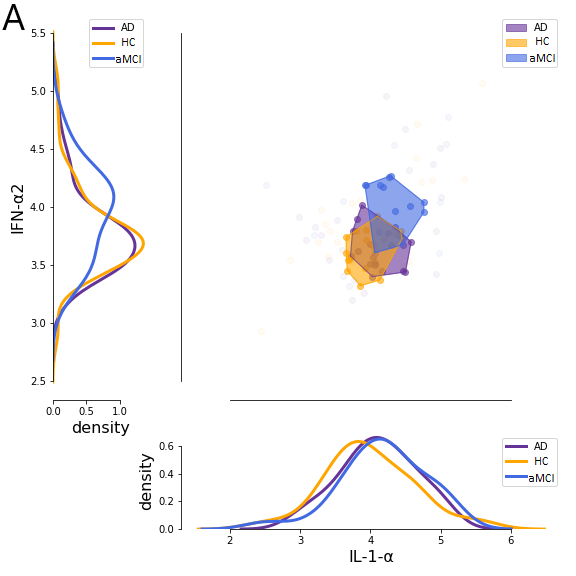
\includegraphics[width=0.45\textwidth]{males.png}
\qquad\qquad
\hspace{1.0cm}
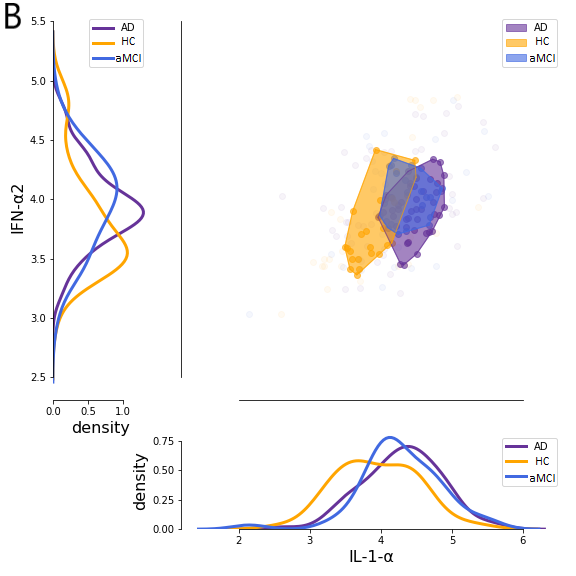
\includegraphics[width=0.45\textwidth]{females.png}
\caption{\textbf{(A)} Scatter plot of IL-1$\alpha$ and IFN-$\alpha$, and distribution plot for the single cytokines along the axes, stratified by diagnostic group (AD, CTL, and MCI) in \textbf{males}.
In this case, the HC group is less separated from aMCI and AD.
\textbf{(B)} Scatter plot of IL-1$\alpha$ and IFN-$\alpha$, and distribution plot for the single cytokines along the axes, stratified by diagnostic group (AD, CTL, and MCI) in \textbf{females}.
In this case, the HC group is well separated from aMCI and AD.
}
\label{fig:cytokine_sex}
\end{figure}

Applying this signature to classify MCI vs CTL samples, it correctly predicted 84.93\% of MCI as \quotes{non-CTL}.
Two cytokines from the signature, IFN$\alpha$2 and IL-1$\alpha$, showed a significant difference between groups also at a single cytokine level in previous analyses.
We plotted them as a representative in all population and stratified the scatter plots by sex (ref Fig.~\ref{fig:cytokine_sex} A, B).
The CTL group resulted better separated from MCI and AD in women as compared with men.
The trajectory of the subject groups moves from CLT to AD, and interestingly the identified signature is able to differentiate MCI from CLT better than from AD.
This is a promising result since it seems more useful to recognize MCI from CLT than full-blown AD from CLT.
Probably the poor sensibility in detecting AD could be linked to the disease evolution that makes nebulous and vague the cytokine pattern in the brain of these patients, as confirmed from several studies that found both up-regulation and down-regulation of many cytokines in AD cerebral samples.
This fact could be more accentuated in our population of old age subjects in which markers of aging are often mixed with those of dementia.

In this study we show that: 1) an easy to get cytokines signature composed of three molecules - IFN$\alpha$2, TNF$\alpha$, and IL-1$\alpha$ - is able to discriminate the studied groups;  2) the combination of IFN$\alpha$2 and IL-1$\alpha$ able to distinguish CTL from  MCI and AD better in women than in men.
Sex (referred to biological differences) and gender (psychosocial and cultural differences) affect human brain biology throughout individual lifespans, affecting male and female cognitive functions differently.
Epidemiological studies show that women have a higher risk of AD as well as a higher dementia prevalence, particularly in the old age, as compared with men.

In conclusion, the identified cytokinome signature shows a good accuracy in differentiating aMCI from CTL, especially in female.
Understanding sex differences will help to define individualized preventive and treatment interventions for AD.

\end{document} % result

\documentclass{standalone}

\begin{document}

\section[Bovine Dataset]{Bovine Paratuberculosis}\label{bovine:bovine}

Paratuberculosis or Johne's disease (JD) in cattle is a chronic granulomatous gastroenteritis caused by infection with \emph{Mycobacterium avium subspecies paratuberculosis} (MAP).
JD is not treatable; therefore the early identification and isolation of infected animals is a key point to reduce its incidence worldwide.
In this work DNetPRO algorithm was applied to RNAseq experimental data of 5 cattle positive to MAP infection compared to 5 negative uninfected controls.
The purpose was to find a small set of differentially expressed genes able to discriminate between infected animals in a pre-clinical phase.
Results of the DNetPRO algorithm identified a small set of 10 transcripts that differentiate between potentially infected, but clinically healthy, animals belonging to paratuberculosis positive herds and negative unexposed animals.
Furthermore, the same set of 10 transcripts differentiate negative unexposed animals from positive animals based on the results of the ELISA test\footnote{
  The enzyme-linked immunosorbent assay.
  It is a common diagnostic tool as well as a quality control check in various bio-medical industries and in medicine.
} for bovine paratuberculosis and fecal culture.
Within the 10 transcripts that together had good discriminative potential, 5 (TRPV4, RIC8B, IL5RA, ERF and CDC40) show significant differential expression between the three groups while the remaining 5 transcripts (RDM1, EPHX1, STAU1, TLE1, ASB8) did not show a significant differences in at least one of the pairwise comparisons.
In conclusion, the discriminant analysis described here identified a set of 10 genes that discriminate between the exposed and sero-converted animals.
When tested in a larger cohort, these finding lead the possible use of RNA expression analysis as new diagnostic test for paratuberculosis.
Such a signature could allow early interventions to reduce the sanitary and economic burden, and to reduce the risk of infection spreading.

In the next sections a description of the dataset and of main DNetPRO results will be discussed.
Further informations can found in the original paper~\cite{Malvisi2019}.

\end{document}
 % Introduction to Bovine
\documentclass{standalone}

\begin{document}

\subsection[Dataset]{Dataset}\label{bovine_data}

Paratuberculosis or Johne's disease (JD) in cattle is a chronic granulomatous gastroenteritis caused by infection with \emph{Mycobacterium avium subspecies paratuberculosis} (MAP).
JD is present worldwide, is a welfare issue and causes significant economic losses.
Cattle are usually infected as young calves but typically do not show clinical signs before 24 months of age, however not all infected animals progress to clinical disease.
JD is not treatable, therefore the early identification and isolation of infected animals, before they start shedding the bacteria, is a key point to reduce its incidence in cattle herds worldwide.
In addition, an association between MAP and Crohn's disease (CD) in humans has been suggested and intensively explored.
Given the economic losses and welfare concerns for livestock, and possible human health risk, the research interest in JD has been driven by the substantial difficulty in early diagnosis of infected animals and the exploration of potentially new diagnostic techniques.

The dataset used in this work was previously discussed and generated by some of the authors of the original paper.
In detail, the dataset used comprised 15036 transcripts from 15 samples, classified as \quotes{serologically negative non exposed cows/healthy} (5 samples, labeled as NN), \quotes{serologically negative exposed cows/ infected} (5 samples, NP) and \quotes{serologically positive cows/clinical} (5 samples, PP).
Only transcripts with non-zero measures for all samples were considered, reducing the dataset to 13529 transcripts.

All data generated or analyzed during this study is available upon request, furthermore all transcript counts per sample are given as supplementary information files of the original paper.


\end{document}
 % Dataset description
\documentclass{standalone}

\begin{document}

\subsection[Results]{Bovine Signature}\label{bovine:bovine_result}

In the context of high-throughput data analysis, a challenge is the search for an optimal choice of variables (a \quotes{signature}) to classify groups of samples or regress trends with optimal performance and minimum dimensionality.
Usually high-throughput omics data (e.g. transcriptomics, ge-nomics, methylomics) provide datasets with few tens to hundreds of samples, and often 1000 times larger numbers of variables.
The objective of dimensionality reduction through the choice of an optimal signature is twofold: 1) the identification of relevant variables, that should separate the signal from the noise (i.e. variables not significantly associated to, or descriptive of the studied process); 2) in a practical context, it is important to establish future diagnostic criteria that can be implemented in cheap and simple toolkits, such as PCR cards or dedicated microarray chips, that usually test a small number of transcripts (ranging from tens to hundreds, at most).
The quantity of samples compared to the available features of this work, join with the final purposes of this kind of analysis, set the well-known ill-posed problem conditions for which the DNetPRO algorithm was thought.

Since the number of sample is drastically small no robust cross-validation procedure can be applied.
So we focused on the identification of a putative gene-signature able to discriminate between NN and NP samples, leaving the PP data as validation set.
In this case we hypothesize that PP samples will be classified more closely with NP sample rather than NN as exposed, possibly infected samples, should be more similar to positive samples, than to negative controls.

\begin{figure}[htbp]
\centering
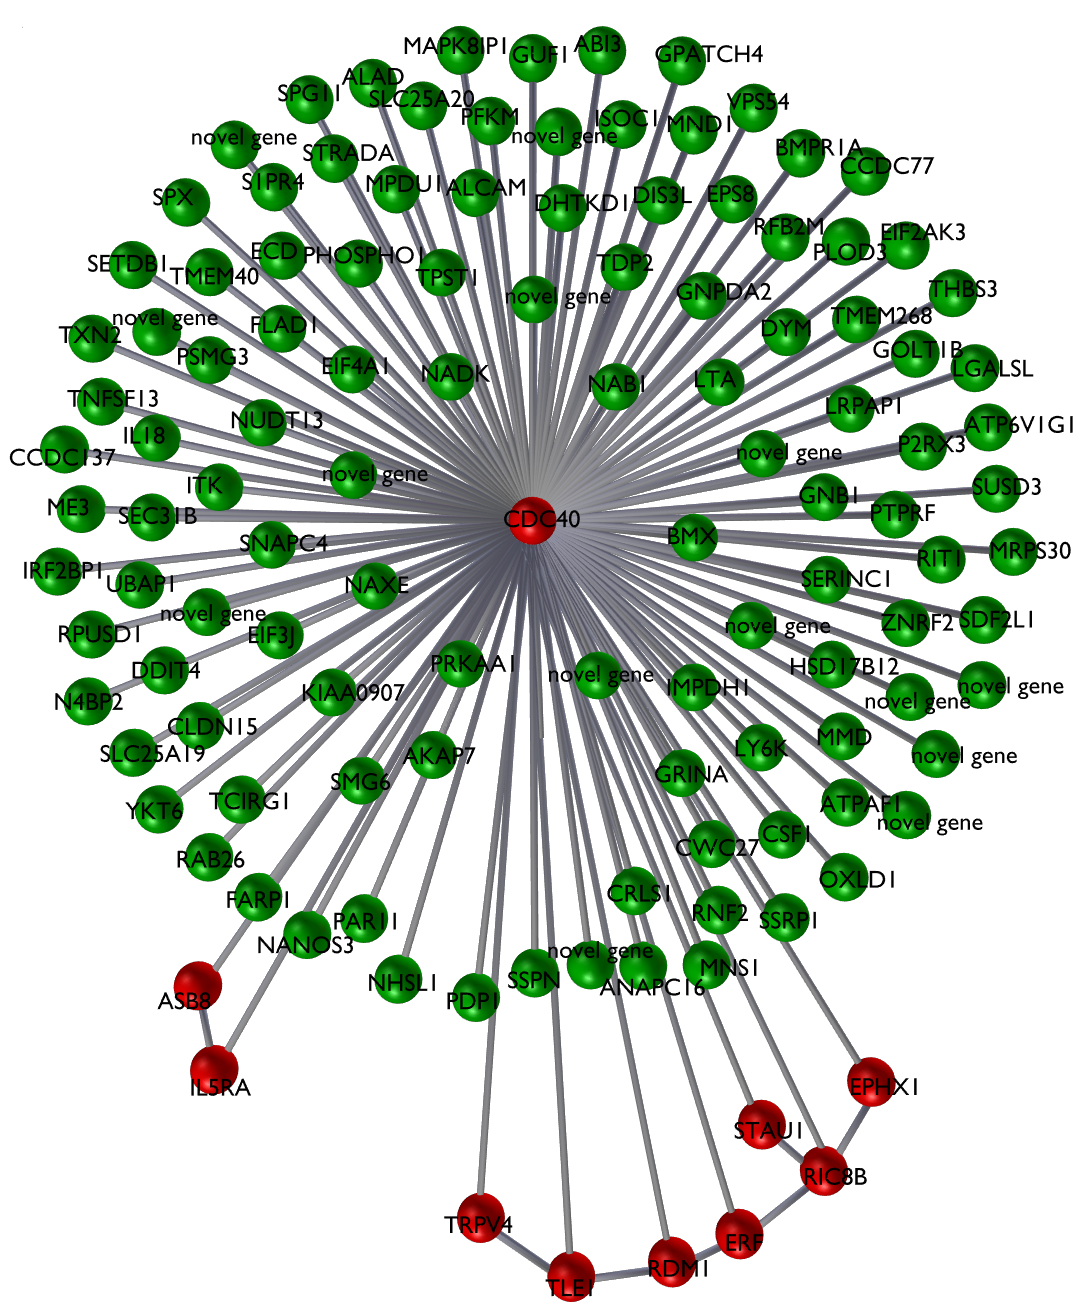
\includegraphics[width=0.4\textwidth]{Bovine_signature.png}
\qquad\qquad
\def\svgwidth{0.45\textwidth}
\input{./img/Bovine_expression_level.pdf_tex}
\caption[Caption Bovine]{(\textbf{a}) Plot of the 123-transcript network, with a details of the 10-probe signature (red nodes)\footnotemark.
(\textbf{b}) Transcript levels for the 10 genes belonging to the classification signature identified by the combinatorial discriminant analysis (CDA).
Some transcripts (EPHX1, RIC8B, IL5RA, ERF, CDC40) show a clear trend  between 5 animals serologically positive to the ELISA test for MAP (PP), 5 exposed serologically negative (NP) and 5 serologically negative unexposed control animals (NN).
}
\label{fig:bovine_signature}
\end{figure}
\footnotetext{
  The figure was generated using a custom network visualizer described in Appendix C - BlendNet.
}


Starting from the top-performing couples of transcripts, we obtained an initial signature of 123 different transcripts (Fig~\ref{fig:bovine_signature}(a), all the nodes), capable to correctly classify 4 out of the 5 NN samples (80\%) and all 5 NP samples (100\% performance).
The average performance was therefore 90\% with Matthews correlation coefficient MCC = 0.82.
Processing the 123-transcript network by removing all pendant nodes (i.e. removing all single transcripts belonging to only one best-performing couple) we obtained a final signature with 10 transcripts with a 100\% performance classifying all NN and NP samples (Fig~\ref{fig:bovine_signature}(a), only red nodes).
As it can be seen, many nodes are directly connected to the central node (belonging to the 10-transcript signature), while only the 10 transcripts of the signature are also connected between each other.

Principal Component Analysis of the 10-transcript signature showed that in many cases there was a progressive increase or decrease in the transcript levels when passing from a healthy (NN) sample to a positive (PP) sample, passing through the infected (NP) sample class.
Fig~\ref{fig:bovine_signature}(b) shows the expression levels of the transcripts belonging to the signature for all samples.

To further validate the goodness of the signature, we generated 10000 different signatures with 10 randomly chosen transcripts, and then applied a Leave-One-Out cross validation procedure to classify all 15 samples with these signatures.
Comparing the performance of the random signatures with the true 10-transcript signature, only 50 of these signatures (corresponding to 0.5\% of the random signature distribution) produced better performance than our signature in terms of classification performance, confirming its high significance.

We even characterized the possible biological role of the signature genes, among the significantly differentially expressed genes, the cell division cycle 40 gene (CDC40) showed the smallest fold change between classes.
However in the identified signature the CDC40 gene is the most central node associated with the health status of the animals related to JD.
CDC40 was also under expressed in the NP and PP groups, compared with the NN group and it has been shown to be involved in clathrin medated endcytosis from a biological point-of-view.
Clathrin is the best characterized coat protein involved in the endocytosis process, specifically in receptor-mediated-internalization.
\emph{Mycobacterium paratuberculosis} enters the host macrophages, its primary target cell, and manages to survive within their phagosome.
It is possible that the under-expression of CDC40 in infected and sick animals compared to unexposed animals may be associate with down regulation of macrophage genes post mycobacterial invasion, facilitating the survival of the pathogen with the host target cell.

Interestingly within the set of 10 discriminating transcripts, in addition to CDC40, others show links with immune response mechanisms, these include IL5RA, ERF and TRPV4.
These genes potentially have functions related to the biology of progression of JD.
Also for the other genes of the final 10-transcript signature a possible biological interpretation related to JD was given (see the original paper for further descriptions).

In conclusion, the DNetPRO algorithm identified a set of 10 genes, the expression levels of which could discriminate between the exposed and sero-converted animals.
These finding lead the possible use of RNA expression analysis as new diagnostic test for JD.
In particular the approach may be able to identify infected animals prior to sero-conversion, prior to a positive ELISA test result.
However, further tests for specificity and validation in a larger cohort are required.


%Description of the bovine dataset with biological background.
%Application of the DNetPRO on the Bovine dataset with the description of the two singatures extracted.
%Discussion on biological interpretation of the genes.

% cite and describe BlendNet repo in the signature figure

\end{document}
 % results and conclusion

\end{document}

% Introduction to feature selection problem and theoretical background. Focus on biological Big Data and problems related.
% Description of the method and efficiency a biological toy model.
% Description of the algorithm implementation with focus on performances of the new implementation.
% Application of the DNetPRO on the Synapse dataset (mRNA, miRNA, RPPA) of Yuan et al. with discussion about obtained performances compared with the most common ML methods and signature characterization
% Application of the DNetPRO on the Cytokine dataset with data description and obtained results
% Application of the DNetPRO on the Bovini dataset with data description and obtained results with biological interpretation


\clearpage


\bibliographystyle{abbrv}
\bibliography{biblio}


\end{document}
